%oneside para una impresi\'on simple.
%titlepage define que vamos a tener una portada.
%openany para que los cap\'{\i}tulos empiecen en cualquier p\'agina y no s\'olo las impares.
%final es para compilar a modo normal. Cambiar a draft para que se compile en modo borrador. No se pone final dado que viene por defecto.
\documentclass[a4paper, 12pt, oneside, titlepage, openany]{book}

% Para el seccionado, debe colocarse al principio este package.
\usepackage{titlesec}

% Encoding + cmap (para obtener un mapeo UTF8 adecuado)
\usepackage{cmap}
\usepackage[utf8]{inputenc}
\usepackage[T1]{fontenc} % Para poder copiar y pegar el texto desde un pdf
\usepackage{lmodern}

\usepackage[table,usenames]{xcolor}

\usepackage[backend=biber, style=iso-authoryear, language=spanish]{biblatex}
\DeclareUnicodeCharacter{202F}{~} % Para reemplazar el caracter 202F por un espacio
\bibliography{biblio.bib}
\setcounter{tocdepth}{3}
\setcounter{secnumdepth}{3}
% Esto último es para la cantidad de niveles en el índice

\DefineBibliographyStrings{spanish}{
  online   = {en línea},
  urlfrom  = {Disponible en:},
  andothers = {\mkbibemph{et\addabbrvspace al\adddot}}
}

\DeclareFieldFormat{urldate}{\mkbibbrackets{consultado\space#1}}

% Para colores (ya incluido en xcolor arriba)
% \usepackage[usenames]{color} % Comentado para evitar conflicto con xcolor

% Para flotar figuras y tablas
\usepackage{framed}

% Para asegurar que las figuras y tablas queden en la secci\'on correspondiente
\usepackage[section,above,below]{placeins}

% Para microtipograf\'{\i}a
\usepackage{microtype}

% Permite tama\~no de fuentes arbitrarios
\usepackage{anyfontsize}

% Itemize
\usepackage{enumitem}
\newlist{Properties}{enumerate}{2}
\setlist[Properties]{label=Propiedad \arabic*.,itemindent=*}
\renewcommand{\labelitemii}{\textasteriskcentered}
\renewcommand{\labelitemiii}{-}

\usepackage{lastpage} % Para poder contar las p\'aginas, habilita el \pageref command.
\usepackage{titleps} % Para la tabla de contenidos
\usepackage{textcase}
\usepackage{pdfpages}

% \parbox[b] es para poner texto sobre el bottom
\newpagestyle{ruled}{
	\sethead{
\includegraphics[width=3.7cm]{./images/UADE_LARGE}}
			{\parbox[b]{0.43\textwidth}{\raggedright\MakeUppercase{Smartstocker: Plataforma de predicción de ventas y optimización de inventario}}} % El parámetro 0.43 puede modificarse para tener más espacio en la columan del medio, y que así el título de la tesis entre mejor.
			{
				\raisebox{1.5ex}{%
					\parbox[b]{0.26\textwidth}{\raggedleft
					\begin{tabular}{r}
						Cano, Nicolás \\
						Venegas, Gabriela
					\end{tabular}
					}
				}
			}\headrule{}
	\setfoot[][][P\'agina \thepage\ de~\pageref*{LastPage}]{}{}{P\'agina \thepage\ de~\pageref*{LastPage}}\footrule{}
	}
\pagestyle{ruled}
% Cambiar el color de la linea divisora:
% \renewcommand\makeheadrule{\color{cyan}\rule[-.3\baselineskip]{\linewidth}{0.4pt}}
% \renewcommand\makefootrule{\color{cyan}\rule[\baselineskip]{\linewidth}{0.4pt}}

% Para que la primera página de cada capítulo no sea tratada como especial
\makeatletter
\let\ps@plain\ps@ruled
\makeatother

% M\'argenes
\usepackage{vmargin}
%\setmarginsrb{leftmargin}{topmargin}{rightmargin}{bottommargin}%
%         {headheight}{headsep}{footheight}{footskip}           %
%Lo ideal ser\'{\i}a lo siguiente
%\setmarginsrb{2.7cm}{4cm}{2.3cm}{2.5cm}{2cm}{0.5cm}{2cm}{0.5cm}
%Pero estos valores se suman, por lo que en realidad ir\'{\i}a asi:
\setmarginsrb{2.7cm}{2cm}{2.3cm}{1.5cm}{0cm}{2cm}{0cm}{1cm}
% M\'argenes, pero otra opci\'on mas acotada
% \usepackage[top=4cm,bottom=2.5cm,left=2.7cm,right=2.3cm]{geometry}

% Seccionado. El par\'ametro left incrementa el margen, lo setteo en 0.
%\titlespacing*{<command>}{<left>}{<before-sep>}{<after-sep>}
% \titlespacing{\section}{0pt}{12pt}{6pt}
%\titlespacing{\subsection}{0pt}{*0}{*0}
%\titlespacing{\subsubsection}{0pt}{*0}{*0}

%Tama\~no de letra de cap\'{\i}tulo y secciones
%\newcommand{\chapfnt}{\fontsize{16}{19}}
%\newcommand{\secfnt}{\fontsize{14}{17}}
%\newcommand{\ssecfnt}{\fontsize{12}{14}}
%\titleformat{\chapter}[display]
%{\normalfont\chapfnt\bfseries}{\chaptertitlename\ \thechapter}{20pt}{\chapfnt}
%\titleformat{\section}
%{\normalfont\secfnt\bfseries}{\thesection}{1em}{}
%\titleformat{\subsection}
%{\normalfont\ssecfnt\bfseries}{\thesubsection}{1em}{}

% Se pide numeraci\'on de tablas en n\'umeros romanos
\renewcommand{\thetable}{\thechapter.\Roman{table}}

%Espaciado antes y despu\'es de una figura respecto del texto
\setlength{\textfloatsep}{5pt}

% Para notas
\usepackage{todonotes}
\setlength{\marginparwidth}{2cm} % El margen es muy estrecho. Esto es solo para solucionar un warning
\newcommand{\Nico}[1]{\todo[color=green!30,inline]{\textbf{Nico:} #1}}
\newcommand{\NicoNI}[1]{\todo[color=green!30]{\textbf{Nico:} #1}}

%Espaciado entre referencias en la bibliograf\'{\i}a
\usepackage{etoolbox}
\patchcmd{\thebibliography}
  {\settowidth}
  {\setlength{\itemsep}{6pt}\settowidth}
  {}{}
\apptocmd{\thebibliography}
  {\small}
  {}{}

\usepackage{tocloft}
\cftsetindents{table}{0em}{4em} % Ajusta 4em seg\'un sea necesario

\usepackage{pdfcomment}
\usepackage[spanish,es-nodecimaldot]{babel}
\usepackage{csquotes}
\addto\captionsspanish{
	\renewcommand{\contentsname}{\'Indice}
	\renewcommand{\listfigurename}{Lista de Figuras}
	\renewcommand{\listtablename}{Lista de Tablas}
	\renewcommand{\tablename}{TABLA}
}

% Para que el primer parrafo de un cap\'{\i}tulo tenga identado.
\usepackage{indentfirst}
\setlength{\parindent}{36pt} %Tama\~no de la identaci\'on.

% Para tablas complejas
\usepackage{multicol,multirow}
\usepackage{array,longtable}

\usepackage{amsmath,amsfonts,amssymb,amsthm}

\allowdisplaybreaks{} % Para que el align permita dividir entre p\'aginas si lo llega a necesitar.

\usepackage{cancel}

\newenvironment{example}[1][Ejemplo]{\begin{trivlist}
	\item[\hspace{\labelsep} {\itshape{} #1}]}{\end{trivlist}}

\newenvironment{examples}[1][Ejemplos]{\begin{trivlist}
	\item[\hspace{\labelsep} {\itshape{} #1}]}{\end{trivlist}}

\newenvironment{EstadoDelArte}
    {\small\begin{center}
    \bfseries{EstadoDelArte} \end{center}}

\newenvironment{Enfoque metodologico}
    {\small\begin{center}
    \bfseries{Enfoque metodologico} \end{center}}

\newenvironment{Cronograma}
    {\small\begin{center}
    \bfseries{Cronograma} \end{center}}

% Para gr\'aficos y figuras
\usepackage{tikz}
\usepackage{graphicx}
\usepackage{wrapfig}
\usepackage{blochsphere}

% Diagramas y figuras.
\usepackage{tikz-cd}
\usepackage{quiver}

% Tablas
\newcommand\titulo[3][\scriptsize]{\rotatebox[origin=c]{90}{\parbox[t]{#2}{\centering #1{#3}}}} % Estos son los t\'{\i}tulos que van al costado de las tablas que tienen todo su contenido sin dividirse.
% \newcommand\rulestitlehalf[1]{\omit\rlap{\parbox{0.3\linewidth}{\centering\textbf{#1}}}}

\usepackage[normalem]{ulem}

\usepackage{setspace}
\onehalfspacing

% En UADE no existe la noción de capítulo en la tesis, por más que en LaTeX sí lo tratemos como tal.
% Además nos piden que el tamaño de letra de lo que para nosotros es una sección, subsección y demás, sean del mismo tamaño.
\titleformat{\chapter}
  {\bfseries\fontsize{14pt}{14pt}\selectfont}
  {\thechapter}{1em}{}
\titlespacing*{\chapter}{0pt}{12pt}{6pt}

\titleformat{\section}
  {\bfseries\fontsize{14pt}{14pt}\selectfont}
  {\thesection}{1em}{}
\titlespacing*{\section}{0pt}{12pt}{6pt}

\titleformat{\subsection}
  {\bfseries\fontsize{14pt}{14pt}\selectfont}
  {\thesubsection}{1em}{}
\titlespacing*{\subsection}{0pt}{12pt}{6pt}

\titleformat{\subsubsection}
  {\bfseries\fontsize{14pt}{14pt}\selectfont}
  {\thesubsubsection}{1em}{}
\titlespacing*{\subsubsection}{0pt}{12pt}{6pt}

% -> Acá se empieza a modificar el tamaño de los títulos autogenerados, como los de las listas de figuras y tablas
\usepackage{tocloft}

\renewcommand{\cfttoctitlefont}{\bfseries\fontsize{14pt}{16pt}\selectfont}
\setlength{\cftbeforetoctitleskip}{12pt}
\setlength{\cftaftertoctitleskip}{6pt}

% Fuente del título (14pt, negrita)
\renewcommand{\cftloftitlefont}{\bfseries\fontsize{14pt}{16pt}\selectfont}
\renewcommand{\cftlottitlefont}{\bfseries\fontsize{14pt}{16pt}\selectfont}

% Espaciado antes y después del título
\setlength{\cftbeforeloftitleskip}{12pt}
\setlength{\cftafterloftitleskip}{6pt}
\setlength{\cftbeforelottitleskip}{12pt}
\setlength{\cftafterlottitleskip}{6pt}


\usepackage[nottoc]{tocbibind}
% IMPORTANTE: En la entrega de UADE se pide en negro, pero visualmente es mejor trabajar con color
\usepackage{hyperref}
\hypersetup{
    colorlinks,
    citecolor=red
}
% Para la entrega de UADE:
%\usepackage[hidelinks]{hyperref}
%\hypersetup{
%    colorlinks=false,
%    pdfborder={0 0 0},
%    linktoc=none
%}

% -> Acá terminamos

\usepackage{mathptmx}

\begin{document}
\clearpage
\thispagestyle{empty}
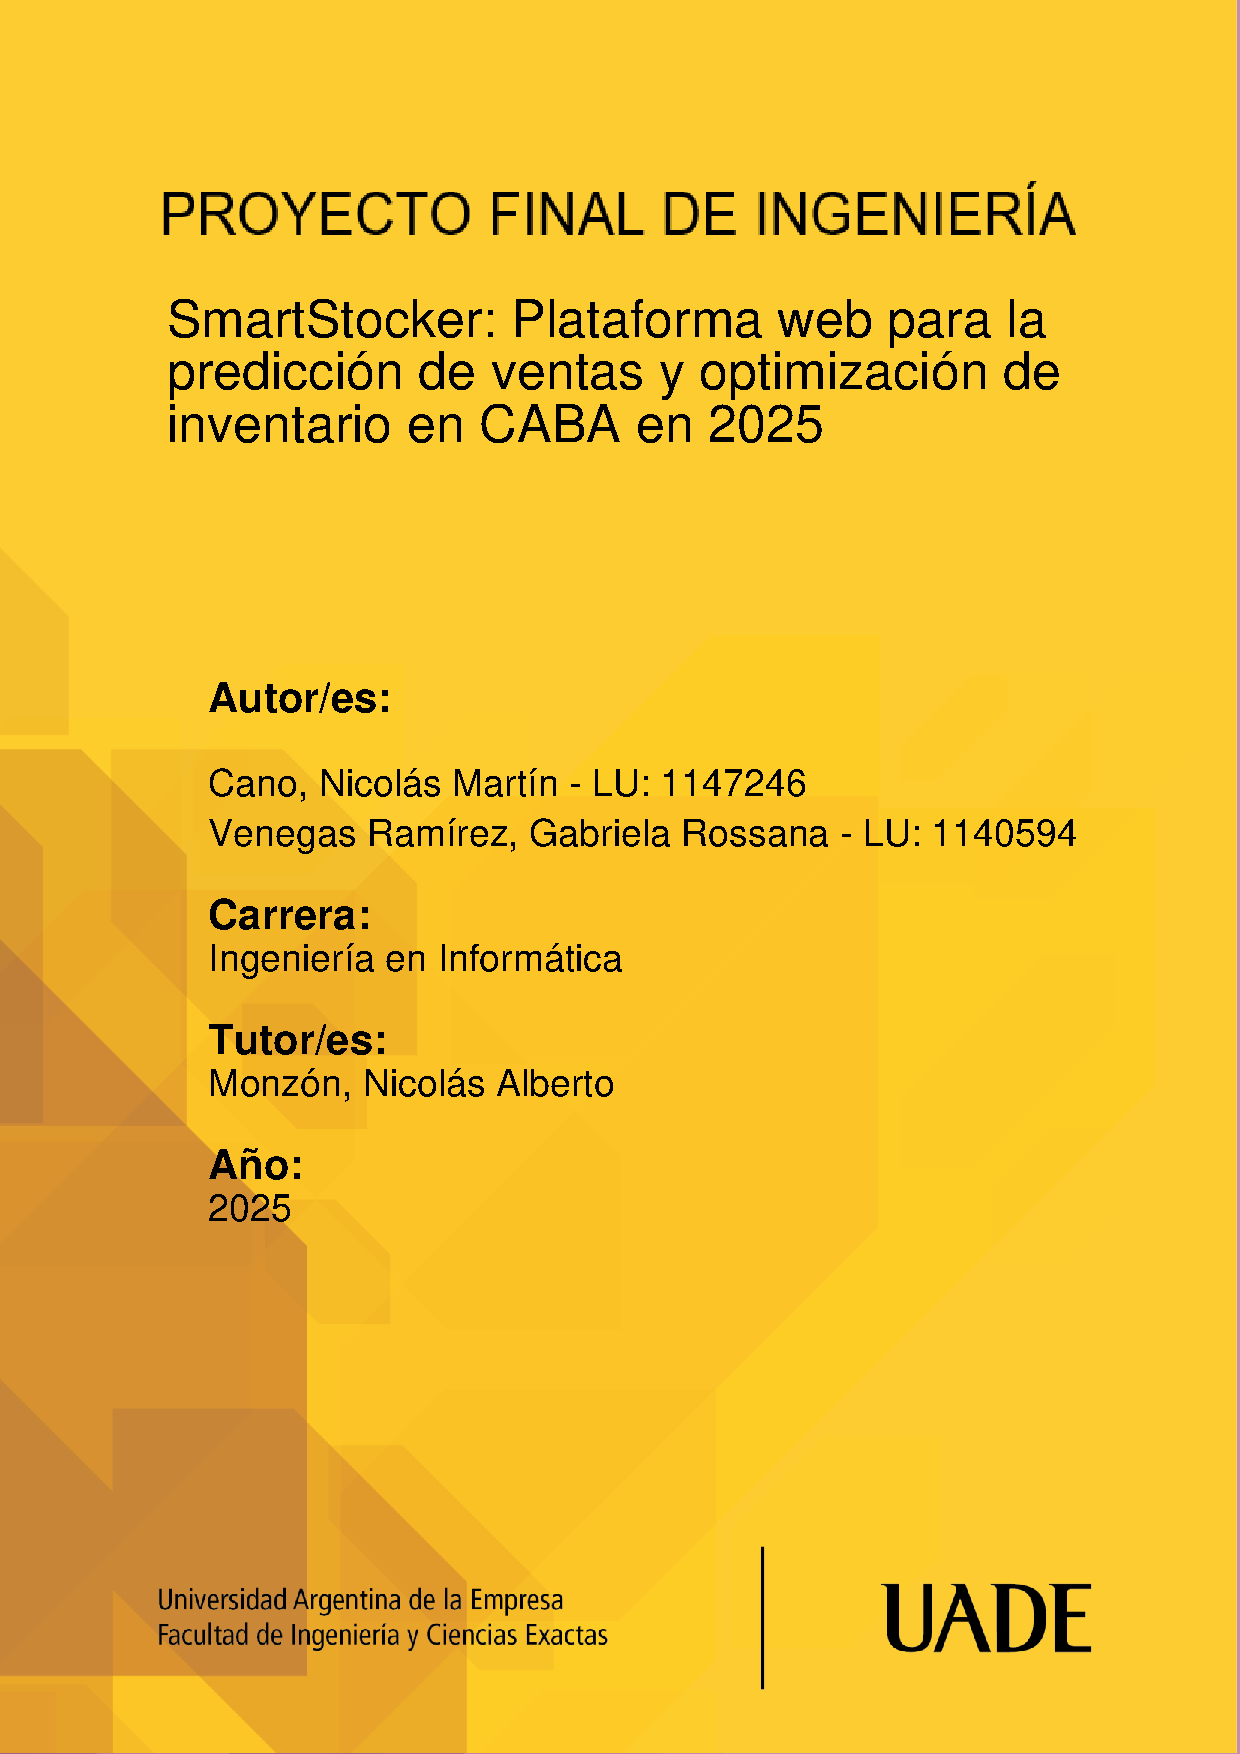
\includepdf[
  pages=1,
  scale=1.01, %1.17
  offset=25mm -25mm,
  pagecommand={\thispagestyle{empty}},
  noautoscale,
  trim=0 0 0 0,
  clip
]{cover/caratula.pdf}
\clearpage
	\begin{titlepage}
    \centering

    {\textbf{\fontsize{18}{20}\selectfont PROYECTO FINAL DE INGENIERÍA} \par}
    \vspace{1.5cm}

    {\textbf{\fontsize{16}{18}\selectfont SmartStocker: Plataforma web para la predicción de ventas y optimización de inventario en CABA en 2025} \par}
    \vspace{0.5cm}

    {\textbf{\fontsize{14}{16}\selectfont Cano, Nicolás Martín -- LU 1147246} \par}
    {\fontsize{14}{16}\selectfont Ingeniería en Informática \par}
    \vspace{1cm}

    {\textbf{\fontsize{14}{16}\selectfont Venegas Ramírez, Gabriela Rossana -- LU 1140594} \par}
    {\fontsize{14}{16}\selectfont Ingeniería en Informática \par}
    \vspace{1.5cm}

    {\fontsize{14}{16}\selectfont Tutor: \par}
    {\textbf{\fontsize{14}{16}\selectfont Monzón, Nicolás Alberto, 
        \\ (UADE) Universidad Argentina de la Empresa, Lima 757, Cdad. Autónoma de Buenos Aires, Argentina.
        \\ (UdelaR) Universidad de la República, Av. 18 de Julio 1968, 11200 Montevideo, Departamento de Montevideo, Uruguay.
    } \par}
    \vspace{3cm}

	{\textbf{\fontsize{14}{16}\selectfont \the\year} \par}
    % {\textbf{\fontsize{14}{16}\selectfont 2025} \par} % se puede hardcodear
	% {\textbf{\fontsize{14}{16}\selectfont \today} \par} % fecha completa si es la entrega final
    \vspace{2cm}

    
\includegraphics[width=0.30\textwidth]{./images/UADE}\par \vspace{1cm}
    {\textbf{\fontsize{14}{16}\selectfont UNIVERSIDAD ARGENTINA DE LA EMPRESA} \par}
    {\fontsize{14}{16}\selectfont FACULTAD DE INGENIERÍA Y CIENCIAS EXACTAS \par}
\end{titlepage}
	%\chapter*{Agradecimientos}

Completar. \sout{Ejemplo de texto tachado}
	\newpage
	%\chapter*{Resumen}

%% Si se quiere enviar este resumen en una p\'agina a alguien, descomentar esto.

%\begin{center}
%\textbf{\large Universidad Argentina De la Empresa}

%\textbf{Facultad de Ingenier\'{\i}a y Ciencias Exactas}

%\textbf{Departamento de Tecnolog\'{\i}a Inform\'atica}

%\end{center}

%\begin{center}
%\large Ingenier\'{\i}a en Inform\'atica
%\end{center}

%\begin{center}
%\textbf{\large Título de la PFI}
%\end{center}

%\begin{center}
%Apellido, Nombres
%Apellido, Nombres
%\end{center}

%\noindent 
Acá va el resumen. \NicoNI{Este es un comentario de margen. Tener en cuenta que el breve margen que tenemos, anula un poco su utilidad. Son libres de usarlo de todas formas}

Con el siguiente comando se imprime el interlineado en el documento pdf. \\
Interlineado simple: 12pt.\\
Interlineado esperado: 18pt.\\
Interlineado exacto de este documento: \the\baselineskip.
	%\newpage
	%\chapter*{Abstract}

This Final Engineering Project proposes the development of a predictive web platform for inventory management in gastronomic establishments in the Autonomous City of Buenos Aires. The main objective is to optimize inventory stock in gastronomic SMEs by 2025 by predicting sales based on a machine learning model, reducing economic losses due to overstocking or shortages, and improving operational efficiency.

The proposal consists of a web platform aimed at gastronomic SMEs, which integrates sales data from platforms like PedidosYa and uses machine learning models to estimate future demand. Unlike existing commercial solutions in the Argentine market, the system allows the incorporation of external variables (weather, holidays) and user feedback to adjust its predictions.

	%\newpage
	\tableofcontents
	\chapter{Introducción}

El sector gastronómico ha sido identificado como un área estratégica dentro de la economía de la Ciudad Autónoma de Buenos Aires, destacándose por su capacidad de transformar barrios a través de la generación masiva de empleos y una variada oferta culinaria, demostrando que esta actividad no solo es fundamental para el turismo, sino también para la vida cotidiana de los residentes del país \parencite{srsur2024gastronomico}. En línea con esta relevancia, la industria gastronómica en Argentina es una de las más dinámicas y resilientes a la situación económica. A pesar de que indicadores de la Cámara Argentina de Comercio y Servicios (CAC) \parencite{cac2024consumo} determinaron que el consumo en el país cerró el 2024 con una caída acumulada de -7,4\%, en el presente el sector gastronómico experimenta un incremento constante que apunta hacia la recuperación. Pero aún cuando tanto empresarios como operadores culinarios han utilizado estrategias financieras y alternativas creativas para tratar de superar las barreras que impone la inestabilidad económica del país, sigue siendo necesario encontrar mecanismos que eleven la eficiencia operativa y así conseguir un punto de equilibrio entre la rentabilidad y la sostenibilidad.

Por lo tanto, ante el panorama presentado los distintos establecimientos gastronómicos buscan la optimización de sus operaciones, apalancándose en soluciones tecnológicas que permitan gestionar aspectos tales como la venta y facturación de sus productos, la gestión de inventario, o análisis y reportes del funcionamiento del negocio, es decir, la tecnología pasa a tener un rol preponderante, ayudando a la toma de decisiones informadas que permitan maximizar la ganancia y reducir los costos  \parencite{agrawal2023predictive}.

En el presente contexto, los avances relacionados a la tecnología predictiva, especialmente aquellos que comprenden modelos de Machine Learning, son capaces de brindar una solución innovadora. Como lo demuestra \parencite{schmidt2022mlsales}, los restaurantes tienen la capacidad de adaptarse a estas invenciones para aprovechar dichos modelos y así predecir la demanda.

A pesar de la implementación exponencial de la informática en múltiples áreas de la industria argentina, la predicción de ventas en el rubro gastronómico sigue sin ser explotada, especialmente por fuera de sistemas propietarios.

Brindarle esta posibilidad a un negocio significa disminuir enormemente la incertidumbre alrededor del cálculo de stock requerido. Esta es una tarea crítica, puesto que comprar por encima de lo necesario, en el caso de los ítems orgánicos con una fecha de vencimiento acotada, se traduce directamente en pérdidas económicas por desperdicio. Y de forma similar, comprar por debajo continúa generando un impacto financiero negativo debido a las ventas que no pueden concretarse, pero también impacta a la reputación del negocio y la fidelización del cliente \parencite{agrawal2023predictive}.

Con fundamento en consultas efectuadas a dueños y encargados de negocios, hoy en día esta es una tarea solamente realizada a partir de la experiencia personal y basada en los datos de ventas de la última semana, no considerando aspectos externos tales como la estacionalidad o el clima, cuando se encuentra demostrado que estos son determinantes a la hora de realizar predicciones en esta industria. \parencite{tanizaki2019forecasting}.

Actualmente, se encuentran dos principales líderes de mercado en Argentina, siendo estos Maxirest y Restô, los cuales a pesar de que brindan soluciones integrales para la gestión del negocio, no atacan esta problemática en particular. Se enfocan únicamente en un análisis descriptivo de las ventas o el inventario, es decir, no abordan de forma específica la problemática de predicción de almacenamiento de stock y por ende tampoco de venta.  

Maxirest es un software integral de gestión gastronómica el cual incluye funcionalidades como reportes en tiempo real, control de inventario y caja, además de ofrecer integración con plataformas de delivery como PedidosYa o Rappi, y medios de pago como MercadoPago o Payway.  

Del mismo modo, Restô es un sistema escalable de gestión gastronómica que facilita la gestión de inventario, compras, cuentas corrientes y emisión de documentos electrónicos. Igualmente, incluye múltiples módulos administrativos y contables, junto con la integración de distintos modos de pago y delivery. 

Sin embargo, ninguno de ellos comprende capacidades de predicción de demanda mediante Machine Learning, ni estimación automática de stock basado en dichas predicciones, así como tampoco permiten el ajuste dinámico del modelo a través de la retroalimentación del usuario. En consecuencia, limitan la capacidad de los negocios para la toma de decisiones basadas en estimaciones futuras, así como tampoco contemplan una personalización avanzada según el contexto de cada local.  

Ante esta situación, se propone la creación de una plataforma web que permita a un negocio, mediante el uso de un modelo de Machine Learning, obtener predicciones de ventas, y del inventario requerido para lograr satisfacerla, es decir, ir un nivel más allá de los líderes del mercado, ofreciendo un análisis predictivo mediante el uso de tecnologías emergentes basadas en Machine Learning \parencite{posch2022bayesian}.

A fin de entrenar el modelo de Machine Learning, se utilizará la información de ventas del negocio, realizando integraciones con los sistemas de POS a fin de obtenerla en tiempo real, y a su vez, se permitirá que el usuario brinde feedback sobre las predicciones, siendo este usado para continuar ajustando el modelo a las particularidades del negocio \parencite{soto2024futuro}.

La solución está orientada a PYMES gastronómicas ubicadas en CABA, que busquen reducir la incertidumbre a la hora de tomar decisiones respecto a la gestión de su stock, utilizando para esto la información de ventas.

\section{Objetivo General}

Permitir la optimización de los niveles de stock en el rubro gastronómico de Argentina en el año 2025, mediante predicción de ventas utilizando un modelo de Machine Learning, en base a la información de ventas, a fin de reducir costos y maximizar ingresos.

\noindent\textbf{Objetivos Específicos:}

\begin{itemize}
    \item Entrevistar a dueños y/o encargados de locales gastronómicos a fin de comprender el proceso de gestión de inventario y qué factores afectan a las ventas.
    
    \item Desarrollar integraciones con sistemas de plataformas de delivery, tales como PedidosYa, a fin de obtener y unificar las ventas en tiempo real.
    
    \item Desarrollar un modelo de Machine Learning que permita pronosticar ventas y extrapolar el inventario mínimo necesario para satisfacer la demanda.
    
    \item Usar fuentes externas de datos, tales como APIs meteorológicas o de feriados, a fin de enriquecer los datos a usar para la predicción.
    
    \item Permitir que el usuario defina alertas que notifique cuando un ítem del inventario queda por debajo de un umbral.
    
    \item Permitir que el usuario brinde feedback sobre estos pronósticos, a fin de permitir que el modelo se ajuste.
    
    \item Desarrollar una plataforma web donde el usuario pueda cargar los productos que vende, indicando de qué elementos del inventario se encuentran compuestos.
\end{itemize}

\section{Alcance}

El proyecto tiene como objetivo el desarrollo de una herramienta integral para la predicción de ventas y gestión de inventario en restaurantes del área de CABA, mediante la integración con sistemas POS, un modelo de Machine Learning y una interfaz web orientada al usuario gastronómico. 

El sistema contempla: 

\begin{itemize}
    \item Integración con sistemas de POS para la recopilación unificada de datos de ventas. 
    \item Desarrollo y entrenamiento de un modelo predictivo de ventas utilizando Machine Learning. 
    \item Incorporación de variables externas y feedback de usuarios en el entrenamiento del modelo. 
    \item Página web para la visualización de ventas, predicciones e inventario. 
    \item Alertas sobre los niveles de inventario. 
\end{itemize}

En el primer release se incluyen los siguientes módulos: 

\begin{itemize}
    \item Módulo de Integración POS (Módulo 1): Desarrolla interfaces para unificar la información proveniente de los sistemas de POS más relevantes en CABA. 
    \item Módulo de Predicción de Ventas (Módulo 2): Entrena un modelo de Machine Learning con datos históricos de ventas y factores externos (clima, feriados, día, etc), considerando el feedback brindado por los usuarios a fin de ajustar aún más el modelo. 
    \item Módulo Web de Visualización (Módulo 3): Permite a los usuarios visualizar ventas históricas, predicciones, niveles de inventario requeridos y brindar feedback sobre las predicciones. 
    \item Módulo de Configuración de Productos (Módulo 4): Permite definir productos, asociar sus componentes de inventario y configurar los umbrales a utilizar por las alertas.
\end{itemize}

Sin embargo, es importante acotar que existen varios aspectos que no son incluidos dentro del alcance del presente proyecto, en vista de la modalidad y características del mismo. No comprende la integración con todos los sistemas POS disponibles, ya que se concentra únicamente en los utilizados dentro del sector gastronómico de CABA. Estos no sufren modificaciones o personalizaciones que alteren su funcionamiento.

Se limita al desarrollo de una plataforma web, por lo tanto, no incluye el diseño de una aplicación móvil o de otro tipo de software adicional. Asimismo, el modelo de Machine Learning se aplica solamente a productos gastronómicos. Por lo tanto, quedan excluidos otros tipos de negocios o productos que, aunque tengan características semejantes, no forman parte de este sector.

	\subsection{Inventario en el rubro gastronómico}

Según \parencite{chopra2019supply}, se define al inventario como el conjunto de bienes o productos que una empresa mantiene en existencia con el propósito de satisfacer la demanda futura. Puede existir en forma de materias primas, productos en proceso o productos terminados, y se mantiene debido a razones como economías de escala, incertidumbre en la demanda o suministro, y variabilidad estacional.

El concepto de \emph{supply chain} se refiere al conjunto de procesos, actores y recursos involucrados en el flujo de productos, información y servicios desde los proveedores hasta el consumidor final. \parencite{chopra2019supply} definen la cadena de suministro como \guillemotleft \emph{todos los niveles involucrados, directa o indirectamente, en satisfacer la demanda del cliente}\guillemotright.

Focalizándose en el rubro gastronómico, esto implica gestionar la compra, almacenamiento y transformación de la materia prima requerida para los distintos productos a comercializar, de forma tal que estén disponibles en el momento que son requeridos, y con los niveles de calidad esperados por el cliente.

 A su vez, existen ciertas particularidades en las materias primas que conciernen a este rubro:

 \begin{itemize}
    \item La demanda es variable, ya que factores externos, tales como el clima o feriados, provocan cambios en el patrón de consumo de los clientes.

    \item Muchas de las materias primas son perecederas, con una vida útil muy corta, lo que implica que las compras a proveedores ocurren muy frecuentemente.

    \item A su vez, los pagos a proveedores tienden a ocurrir al menos una semana luego de la entrega de mercadería, lo que implica que cualquier desvío, ya sea en cantidad o tipo de materia prima requerida se traslada directamente como una pérdida económica, debido a la naturaleza perecedera de la misma.
\end{itemize}

Este proceso de reposición de inventario, siendo uno de los que ocurre con mayor frecuencia, es a su vez uno de los de mayor costo asociado, significando para uno de los entrevistados, en mayo de 2025, alrededor de 6 millones de pesos argentinos por semana en cada uno de sus locales.

A su vez, el estimar cuanto se deberia comprar es una tarea que hoy en día, debido a los costos asociados, queda en manos del personal con mayor conocimiento del negocio. Inclusive, muchas veces recae directamente en el dueño, quien debe considerar no solo las ventas que ya ocurrieron, sino también cómo los factores externos, como los feriados, el clima y el momento del mes, podrían influir en las ventas de la próxima semana.

\subsection{Aprendizaje supervisado}

El aprendizaje supervisado es una de las principales ramas de Machine Learning y se refiere al proceso mediante el cual un algoritmo aprende a realizar predicciones a partir de un conjunto de datos (dataset) etiquetado. Según \parencite{russell2022ai}, \guillemotleft{}\emph{en el aprendizaje supervisado, el agente observa pares de entrada-salida y aprende una función que mapea desde la entrada hacia la salida. Por ejemplo, las entradas podrían ser imágenes de una cámara, cada una acompañada de una salida que indica \textquotedblleft autobús\textquotedblright{} o \textquotedblleft peatón\textquotedblright{}. Esta salida se llama etiqueta. El agente aprende una función que, dada una nueva imagen, predice la etiqueta apropiada.}\guillemotright{}.

Formalmente, el aprendizaje supervisado parte de un conjunto de entrenamiento conformado por $n$ ejemplos etiquetados:

\[(x_1, y_1), (x_2, y_2), \ldots, (x_n, y_n)\]

\noindent donde cada $x_n$ es una entrada (también conocida como vector de características) y cada $y_n$ es la salida o etiqueta correspondiente. Estos ejemplos son generados por una función desconocida $f(x)$, y el objetivo del algoritmo es encontrar una función aproximada $h(x)$, denominada \emph{hipótesis}, que generalice correctamente sobre datos no vistos.

Los problemas que son abarcados por este tipo de aprendizaje son

 \begin{itemize}
    \item Clasificación: cuando las salidas $y_n$ son categorías discretas, tales como un tipo de producto o la decisión de si realizar o no una compra.

    \item Regresión: cuando las salidas son valores numéricos continuos (por ejemplo, predicción de precios, estimación de demanda o ventas futuras).
\end{itemize}

El problema de predicción de ventas abarcado en esta tesis entra en la categoría de problemas de regresión, ya que la variable a predecir es numérica continua.

\subsection{Métricas}

A la hora de implementar algún algoritmo predictivo, es fundamental tener la capacidad de medir cuán precisas son las predicciones devueltas. Es aquí, donde las métricas toman un rol preponderante, ya que permiten evaluar de distintas formas la performance de un algoritmo.

Para el caso específico de regresión, se utilizan métricas que calculan el grado de error entre los valores reales y los valores predichos por el modelo

Basándonos en \parencite{hyndman2018forecasting, james2013isl} podemos pasar a definir las tres métricas principales para modelos de regresión.

\begin{itemize}
    \item \textbf{MAE (Mean Absolute Error)}: Mide el promedio de las diferencias absolutas entre los valores predichos por el modelo y los valores reales observados, sin considerar la dirección del error. La unidad utilizada es la misma de lo que se está prediciendo, lo que facilita su interpretación, y es menos sensible a valores atípicos en comparación con otras métricas como MSE y RMSE. Se define como:

    \[
        \mbox{MAE} = \frac{1}{n} \sum_{t=1}^{n} \left| y_t - \hat{y}_t \right|
    \]

    \item \textbf{MSE (Mean Squared Error)}: Cuantifica la diferencia promedio entre los valores reales observados y las predicciones de un modelo. Se calcula como el promedio del cuadrado de los errores, es decir, la diferencia entre los valores reales y los valores predichos. Es muy sensible a valores atípicos, y su unidad es el cuadrado de la unidad de error original, lo que hace que no sea de fácil interpretación.
    
    \[
        \mbox{MSE} = \frac{1}{n} \sum_{t=1}^{n} \left( y_t - \hat{y}_t \right)^2 
    \]

    \item \textbf{RMSE – Root Mean Squared Error:} Similar al MSE, penaliza de igual forma a los valores atípicos, pero al aplicar una raíz cuadrada al error permite que este se mantenga en la misma escala que las unidades originales, solucionando el problema de interpretación del MSE.

    \[
        \mbox{RMSE} = \sqrt{ \frac{1}{n} \sum_{i=1}^{n} (y_i - \hat{y}_i)^2 }
    \]
\end{itemize}

\subsection{CatBoost}

Antes de definir el algoritmo CatBoost, es necesario definir dos conceptos claves para comprenderlo, siendo estos el concepto de función de pérdida, y de Gradient Boosting.

Una \emph{función de pérdida} es una función matemática que cuantifica el error entre la predicción del modelo ($\hat{y}$) y el valor real observado ($y$). Su objetivo es proporcionar una medida numérica del desempeño del modelo para cada ejemplo individual o conjunto de datos, la cual puede luego utilizarse para optimizar los parámetros del modelo mediante técnicas como el descenso del gradiente.

Formalmente, dada una función de predicción $f(x)$ y un valor objetivo $y$, una función de pérdida $L(y, f(x))$ devuelve un valor escalar que representa la penalización por la discrepancia entre ambos.

Definido el concepto de función de pérdida, podemos pasar a explicar el concepto de Gradient Boosting, siendo este una técnica de ensamble supervisado que construye un modelo predictivo fuerte mediante la combinación secuencial de múltiples modelos débiles, generalmente árboles de decisión, con el objetivo de corregir los errores residuales del conjunto anterior. A cada paso, el nuevo modelo es entrenado para minimizar el error del conjunto previo, utilizando métodos de optimización basados en el gradiente de una función de pérdida.

En este caso, la función utilizada por CatBoost es RMSE, cuya fórmula matemática ha sido definida previamente

Dada la definición de Gradient Boosting, podemos pasar a explicar CatBoost (Categorical Boosting), definido en \parencite{dorogush2018catboost}, como uno de los algoritmos implementados con esta técnica. Está diseñado específicamente para manejar datasets que contienen una combinación de variables numéricas y categóricas, destacándose por su capacidad para procesar variables categóricas sin necesidad de codificación previa (como one-hot o label encoding), y de reducir el overfitting que ocurre durante el entrenamiento mediante una técnica llamada Ordered Boosting. 

A su vez, es uno de los algoritmos de Machine Learning más performantes a la hora de trabajar con datasets de las características a utilizar en esta tesis.
	\chapter{Estado del Arte}\label{chapter03}

Según \parencite{creswell2014}, el estado del arte constituye una instancia fundamental dentro del proceso de investigación debido a que permite conocer las soluciones vigentes a la problemática abordada, identificar los aportes realizados por otros actores y a su vez delimitar las distintas oportunidades de innovación para el proyecto en curso.

En este sentido, el presente apartado desarrolla un análisis del estado del arte en relación con el diseño de soluciones tecnológicas orientadas a la gestión inteligente del stock en el sector gastronómico, haciendo énfasis en aplicaciones que incorporan técnicas de \emph{Machine Learning} para la predicción de la demanda.

Ahora bien, con el objetivo de identificar los aportes diferenciales de la solución propuesta, se abordan tres tópicos esenciales: primeramente aplicaciones comerciales actuales, en segundo lugar proyectos académicos o experimentales relacionados, y por último una lectura estratégica basada en la teoría del Océano Azul para identificar oportunidades de innovación y creación de valor en espacios de mercado poco explorados.

\section{Soluciones tecnológicas con enfoque predictivo en el sector gastronómico internacional}\label{sec:estado-internacional}

A nivel mundial, la búsqueda por una gestión eficiente de los establecimientos gastronómicos ha impulsado el desarrollo de herramientas que integran inteligencia artificial, especialmente técnicas de Machine Learning. Estas soluciones han surgido en distintos países con el objetivo de anticipar la demanda y optimizar la administración de insumos. A continuación, se presentan dos de las plataformas más relevantes, con el fin de profundizar en el uso de la inteligencia artificial en el sector gastronómico a nivel global.

\begin{itemize}
    \item \textbf{5-Out}. Plataforma estadounidense que utiliza \emph{Machine Learning} para predecir ventas con integración de fuentes internas (TPV, programación de personal, reservas) y externas (clima, eventos), habilitando recomendaciones de compra para equilibrar inventario y reducir desperdicio. Es integrable con sistemas como Toast, Square y 7Shifts; además, anunció una alianza con Craftable para ampliar funciones administrativas y financieras \parencite{fiveout2025partnership}.

        Gracias al análisis predictivo, esta herramienta puede indicarle de forma detallada al sitio gastronómico la cantidad de productos que deberá comprar para mantener un equilibrio en la gestión del inventario. Esto ayuda a reducir significativamente el desperdicio de alimentos y aumenta en consecuencia la rentabilidad. 

        Además, esta aplicación es compatible e integrable a sistemas actuales como Toast, Square y 7Shifts, y consideran unirse a Craftable para sumar funciones administrativas y financieras a sus capacidades predictivas como alternativa innovadora en la gestión de restaurantes. 

    \item \textbf{Restoke}. Es una startup australiana que automatiza procesos administrativos en restaurantes mediante IA: control de inventario y compras, programación y proyección de ventas, e integración con POS y software contable. En 2024 fue noticia por su crecimiento y una ronda de financiación de USD 5,1 millones, con casos reportados de fuertes reducciones de costos operativos \parencite{santoreneos2024restoke}.
\end{itemize}

\subsection{Soluciones comerciales actuales en el sector gastronómico argentino}\label{sec:estado-arg}

Actualmente, en Argentina, el mercado del software especializado en el sector gastronómico se encuentra en constante crecimiento, que si bien todavía no ha explotado el mundo del aprendizaje automatizado, dispone de herramientas que facilitan la administración y operación diaria de distintos establecimientos como restaurantes, sitios de comida rápida, cafés y lugares afines. Es por esto que se resalta algunas de las plataformas más utilizadas dentro del presente rubro, Maxirest y Restô , ambas con un enfoque integral en la gestión del negocio.

\begin{itemize}
    \item \textbf{Maxirest} \parencite{latam2024maxirest}. Se trata de una herramienta reconocida en el mercado por su robustez y funcionalidad. Su enfoque se centra exclusivamente en el análisis descriptivo de datos históricos y es una de las soluciones más consolidadas del país en el ámbito gastronómico. La plataforma permite automatizar diversas tareas operativas, tales como la gestión de cocina, la toma de pedidos, la administración de reservas e inventario, y la generación automática de reportes. Además, incluye un módulo específico para delivery y takeaway, lo que resulta especialmente relevante considerando que el 47,6\% de las ventas del sector se realizan a través de estas dos modalidades.
    
    \item \textbf{Restô} \parencite{iprofesional2014resto}. Es un sistema de gestión gastronómica que forma parte del ecosistema del software Tango, el cual fue desarrollado por la empresa argentina Axoft. El propósito de este es brindar una solución a la necesidad de una herramienta tecnológica que simplifique los procesos del día a día de dicho sector. En línea con dicho objetivo, este brinda una administración integral en múltiples establecimientos gastronómicos con diversas funciones tales como la gestión de mesas y reservas, el control de stock de insumos, la facturación electrónica, el seguimiento de ventas, y muchas otras más. De igual manera, gracias a su enfoque modular y adaptable, es utilizado tanto por pequeños comercios como por grandes cadenas gastronómicas, lo que le ha permitido posicionarse como una de las soluciones locales más completas del mercado para la administración de negocios del rubro alimenticio.
\end{itemize}

\subsection{Propuestas académicas y experimentales}\label{sec:academico}

Aunque el modelo predictivo se ha desarrollado en investigaciones de múltiples áreas, existen escasos trabajos académicos enfocados específicamente en el rubro gastronómico. Uno de ellos es \parencite{hari2024predictiwaste}: \emph{PredictiWaste: An ML-Powered Framework for Sustainable Food Inventory Optimization in Restaurants (marco de trabajo basado en aprendizaje automático para la optimización sostenible del inventario de alimentos en restaurantes)}, se introduce un modelo de análisis predictivo para reducir el desperdicio de alimentos en el inventario y la planificación de menús de restaurantes. 

Por consiguiente, realiza el pronóstico del desperdicio basándose en factores como el tipo y cantidad de alimento, número de comensales, tipo de evento, condiciones de almacenamiento, historial de compras, métodos de preparación, estacionalidad, ubicación y precio. El sistema clasifica el desecho como mínimo, moderado o alto y sugiere medidas de control de inventario, ayudando en consecuencia a las empresas a optimizar sus recursos y a promover la sostenibilidad. 

Igualmente, una de las propuestas más representativas se encuentra en \parencite{schmidt2022mlsales}, con el pronóstico de ventas de restaurantes basado en aprendizaje automático. Este estudio afirma que para la correcta gestión del personal en los restaurantes, es necesaria la previsión precisa de las ventas, y propone un caso práctico sobre diversos modelos de aprendizaje automático utilizando data real de las ventas de un negocio, tipo restaurante de tamaño medio, y la inclusión de modelos de redes neuronales recurrentes de tendencia para la comparación de su rendimiento a través de diversos métodos.

De la misma manera, otros estudios como el \parencite{tanizaki2019forecasting} sobre la previsión de la demanda en restaurantes mediante aprendizaje automático y análisis estadístico, construyen un modelo específico para cada tienda física que combina funcionalmente datos de diversos factores externos tales como ubicación, clima y eventos, mediante aprendizaje automático, para luego analizar el resultado de verificación con datos de otros negocios similares.

\subsection{Océano Azul}

La Estrategia del Océano Azul es una teoría innovadora conceptualizada en \parencite{kim2015estrategia} que redefine la competencia empresarial a través de la innovación, como creadora de oportunidades y crecimiento rentable en mercados inexplorados.

Según sus autores, los océanos rojos representan a todas las industrias que hoy operan en el mercado, donde sus características están altamente definidas y son aceptadas, lo que conlleva a la lucha entre empresas rivales por obtener el posicionamiento ventajoso de llevarse una mayor participación en la demanda existente. Es decir, es un nivel de subsistencia toda vez que al saturarse el mercado se reducen las perspectivas de rentabilidad y sostenibilidad, lo que ocasiona que los productos pierdan su rasgo de distinción y por ende se conviertan en genéricos.

Por el contrario, los océanos azules representan nichos de mercado no explorados donde es factible la creación de demanda con un crecimiento altamente rentable. En el contexto de los océanos azules, la competencia carece de relevancia, dado que los parámetros operativos aún no han sido definidos.

Los teóricos con la intención de cuantificar el impacto de la creación de los océanos azules sobre el crecimiento de una compañía, analizaron el lanzamiento de 108 negocios nuevos, lo que arrojó como resultado que el 86\% eran extensiones de líneas existentes, es decir, pertenecientes al océano rojo y el 14\% restante de los lanzamientos pertenecientes a océanos azules.

Esto subraya la diferencia entre la creación de nuevos mercados sin competencia que rompen el equilibrio tradicional entre valor y costos, generando crecimiento empresarial con ganancias más rentables y a su vez con la competencia tradicional directa en mercados ya existentes que se encuentran saturados por parte de empresas que luchan por el control de la demanda.

En la estrategia del océano azul, se definen como varias herramientas fundamentales a saber, la matriz de \emph{Eliminar-Reducir-Aumentar-Crear} como recurso central, que \guillemotleft obliga a las compañías no solo a perseguir simultáneamente la diferenciación y el bajo costo, sino también a romper con el compromiso de valor-costo. No se trata de crear una nueva curva de valor por crearla, sino de identificar las variables correctas que transformarán la dinámica de la industria.\guillemotright \parencite{kim2015estrategia}.

Este enfoque analítico desafía la lógica de la competencia tradicional de la industria brindando apertura a nuevos paradigmas de análisis económico, ya que impulsa a las empresas a pensar de manera diferente sobre cómo crear valor para el cliente. 

Ahora bien, la Matriz \emph{Eliminar-Reducir-Aumentar-Crear}, es la representación tabular del Marco de las Cuatro Acciones, y tiene como finalidad ayudar en la formación de las ideas para que la toma de decisiones tenga como objetivo la diferenciación y el bajo costo de manera integrada.

Asimismo, otra herramienta fundamental es la \emph{Curva de Valor}, la cual permite una visualización gráfica del perfil estratégico de una empresa en relación con los factores clave de la industria. Esta curva permite identificar si una propuesta se encuentra alejada o no, de lo convencional, permitiendo así la detección temprana de oportunidades de innovación que generen una ventaja competitiva sostenible dentro del mercado.


\subsection{Matriz ERAC}\label{sec:erac}

\begin{figure}[htbp]
    \centering
    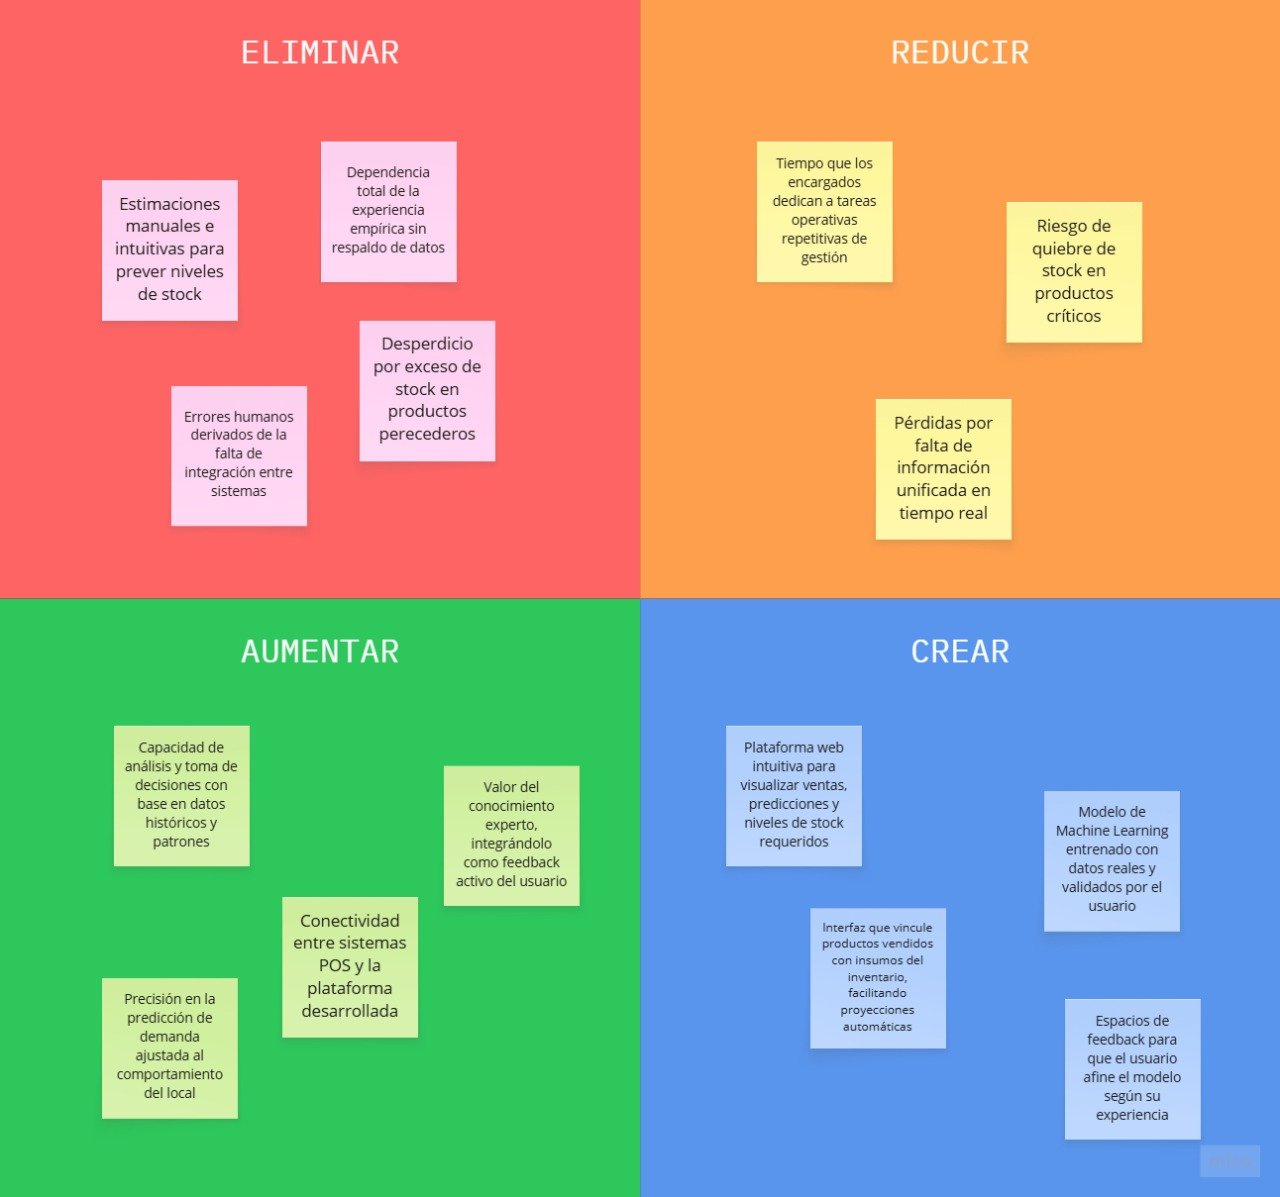
\includegraphics[width=0.7\textwidth]{images/matrizEric.jpeg}
    \caption{Matriz ERAC de SmartStocker}
    \label{fig:eric}
\end{figure}

Las variables identificadas en la matriz ERAC (Fig.~\ref{fig:eric}) se utilizan como insumo para construir la Curva de Valor (Fig.~\ref{fig:curva}), con el objetivo de visualizar el posicionamiento de \emph{SmartStocker} en relación con sus competidores en el mercado.

\FloatBarrier

\clearpage
\subsection{Curva de Valor}\label{sec:curva-valor}

\begin{figure}[htbp]
    \centering
    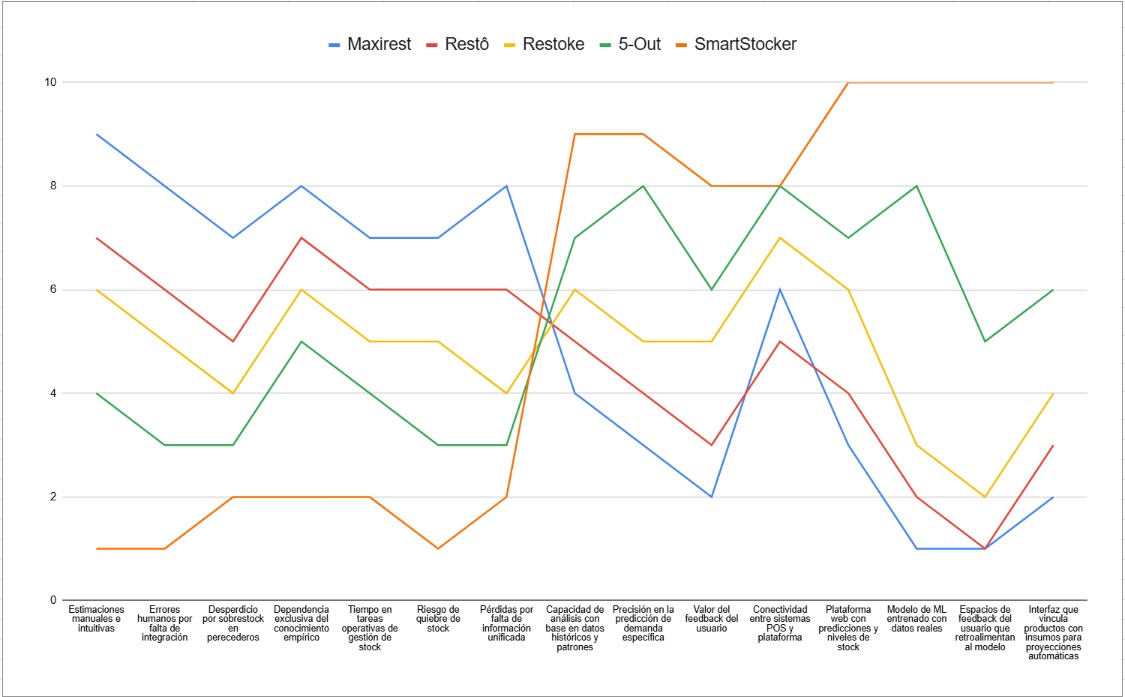
\includegraphics[width=0.7\textwidth]{images/curvaValor.jpeg}
    \caption{Curva de valor}
    \label{fig:curva}
\end{figure}

\FloatBarrier

\subsection{Síntesis}\label{sec:sintesis-estado}

Una vez realizado el análisis del estado del arte y de las herramientas que utiliza, se evidencia el diferencial del presente proyecto ya que no existen en la actualidad soluciones tecnológicas predictivas en el mercado nacional que conduzcan a una precisa gestión del inventario en el rubro gastronómico en base a la información de ventas, toda vez que las otras plataformas en el mercado se limitan a funciones descriptivas, basadas en estadísticas generales de consumo.

Asimismo, la presente tesis desarrolla un enfoque novedoso ya que utiliza el modelo de Machine Learning para predecir las cantidades de producto necesarias para el funcionamiento óptimo del usuario, ajustar los niveles de existencias en tiempo real y mantener los niveles de stock necesarios para que el local sea altamente productivo y su rentabilidad sea sostenible.

Mantener el inventario en un punto de equilibrio óptimo impacta directamente en la eficiencia operativa del negocio ya que implica la reducción de costos y la posibilidad de minimizar el capital inactivo en productos consumibles. Como consecuencia, genera grandes beneficios tales como el control de los desperdicios que puede traducirse a corto plazo en una reducción de gastos. Permite la rotación correcta de los insumos, evita la sobrecompra y la posible merma por caducidad ya que los alimentos tienen un tiempo de vida útil limitado, y luego de transcurrido este, no queda otra que descartarlos por control sanitario. Consecuencialmente, también se evita el gasto colateral que se genera en tiempo horas-hombre en personal utilizado para eliminar desechos, asear y reacondicionar el lugar.

Además, permite determinar el stock de seguridad, lo que es igual a la cantidad mínima de insumos necesarios para la producción base del negocio, facilitando así la gestión de mantenimiento de los volúmenes necesarios con el fin de evitar posibles rupturas en la cadena de suministro, ya que puede establecerse de manera certera el punto de pedido en el que es necesario emitir una orden de compra. 

Cabe resaltar que un exceso en los niveles de inventario es negativo para negocios con espacios limitados lo que puede conllevar al inadecuado uso de algunos productos con fecha cercana a la caducidad como medida de aprovechamiento de la materia prima, esto disminuye el nivel del servicio y por ende la competitividad del negocio.

En consecuencia, favorece la gestión de compras, evitando la adquisición urgente de materiales específicos necesarios para la elaboración de platos, por lo que asegura la disponibilidad constante de insumos para la totalidad del menú y garantiza la integridad de la oferta gastronómica, que es la principal fuente de ingresos del usuario. Evita además cambios abruptos en los stocks que podrían afectar el nivel de servicio como elemento esencial y diferenciador de la competencia y que además conforman una parte importante de los lineamientos estratégicos de la empresa para que su productividad sea sostenible.  

Dada la inexistencia de un sistema de gestión de stocks con un modelo predictivo en base a la información de ventas, el presente trabajo es una herramienta innovadora en el área gastronómica para aquellos negocios que desean aumentar su capacidad de  producción a través del manejo eficiente de su reabastecimiento.

Por otro lado, uno de los factores más importantes del costo de las operaciones empresariales está relacionado con el capital  invertido en la reposición de inventario necesario para el funcionamiento del local, el cual al quedar cautivo anula cualquier posibilidad de reinversión directa o de un nuevo destino generador de rentabilidad y posicionamiento.

En esta medida, dada la inmovilidad del capital, es determinante tomar decisiones que reduzcan costos, con lo cual surge la necesidad de regular los niveles de stock de los productos, cuantificarlos y gestionar su reposición. Aunque los inventarios almacenan valor, pueden generar una pérdida irrecuperable para el usuario cuando hay sobreabastecimiento, todo esto debido a que absorben el capital que podría estar disponible para otras opciones de inversión, sin embargo, lo paralizan y hasta pueden generar pérdidas cuando los consumibles se vencen o deterioran. También es importante la administración del espacio, ya que un stock superior al que puede ser preservado o refrigerado puede deteriorar sus componentes y por ende se podría ver afectada la calidad del producto final.

En otro sentido, disponer de pocos insumos genera una pausa considerable en la producción y  desmejora la calidad del producto ofrecido en el menú, lo que podría traducirse en el aumento de los costos por la carencia de artículos en el momento de ser demandados, pérdida de los beneficios originados de la venta imposible y el deterioro de la imagen comercial de la empresa, impulsando finalmente al consumidor a adquirir el bien a través de la competencia. Esta negativa también está asociada con la demora a la hora de satisfacer la demanda de pedidos al  momento en que son solicitados. 

Por otro lado, debe considerarse el análisis de la ventas como un factor fundamental para determinar la logística que deberá emplear la empresa para la reposición de inventario y así establecer su modelo de gestión. La predictibilidad entonces estará determinada por elementos probables y no por factores aleatorios, ya que la toma de decisiones se hará en función de estadísticas fidedignas arrojadas por el sistema alimentado con datos actualizados proporcionados por el usuario.

En consecuencia, la solución propuesta en esta tesis sobre la optimización de los niveles de stock en el rubro gastronómico de Argentina en el año 2025, utilizando modelos de Machine Learning para predecir los niveles requeridos en base a la información de ventas, resulta técnicamente factible y presenta un concepto innovador en gestión empresarial ya que pretende optimizar mecanismos de producción a través de la predictibilidad. Se configura en una herramienta avanzada para los propietarios de restaurantes y negocios afines, quienes a través de su implementación podrán obtener notables beneficios en cuanto a productividad y rentabilidad. Por último, el presente trabajo representa la oportunidad de crear un nuevo nicho de mercado en Argentina, específicamente la Ciudad Autónoma de Buenos Aires, basado en la innovación tecnológica por medio de la toma de decisiones informadas sustentadas en estadísticas proporcionadas por el mismo usuario.  


\section{User research}\label{sec:user-research}

\subsection{Entrevistas}\label{sec:entrevistas}

Durante la etapa de descubrimiento del proyecto se consideró fundamental realizar entrevistas cualitativas con el fin de comprender a profundidad las múltiples dificultades que se enfrentan actualmente en la administración de negocios gastronómicos, buscando indagar tanto en las dinámicas como en los patrones diarios dentro del sector, especialmente en la gestión de inventarios y su impacto sobre dichos negocios.

Primeramente se entrevistó a Ulises Litterio, dueño de La Brava Burguer, la cual es una cadena gastronómica que consta de tres locales y 25 empleados. Se centra en la venta de hamburguesas y llevan a cabo todas las actividades correspondientes para el mantenimiento y desarrollo de calidad de las mismas que van desde la compra de materias primas hasta la venta final de estas con delivery propio. Ahora bien, el control del inventario se encuentra descentralizado, básicamente cada jefe de cocina realiza un conteo el cual se le informa al encargado, quien lo carga en una planilla de Excel que luego es revisada por el dueño (Ulises Litterio). Además, todas las compras necesarias son realizadas de manera semanal, aunque pueden repetirse en distintos momentos de la semana si hay productos o ingredientes faltantes.

El cálculo de reposición de stock se basa en datos como las ventas semanas anteriores, fechas clave, como feriados, y la intuición de los trabajadores sobre la demanda esperada. Sin embargo, gestionar el inventario de esta manera conlleva una alta tasa de error tanto por sobrestock como por faltantes, lo cual genera desperdicios tanto a nivel económico como alimenticio. Además, Ulises destaca la dificultad de consolidar datos de ventas debido a que operan con múltiples plataformas de delivery como Rappi y PedidosYa, cada una con su propio sistema individual, y aunque ha considerado la opción de emplear un software como MaxiRest, ha terminado por descartar dicha idea debido a los costos elevados que tendría que pagar.

En segundo lugar, se entrevistó a Oscar Campione, dueño de una rotisería familiar que opera con un único local instalado en una parte de la casa. La venta del negocio se basa única y exclusivamente en por delivery propio a través de PedidosYa. Además el personal se encuentra compuesto por cuatro personas los cuales son todos integrantes de la familia, exceptuando al repartidor.

Su modalidad de trabajo actualmente consiste en preparar y vender productos del mismo día, llevando manualmente un control de las mismas al finalizar la noche, de tal manera que el cálculo de reposición se hace constantemente para a la mañana siguiente reponer solamente lo vendido. Esta modalidad los expone a constantes errores que pueden afectar significativamente los costos para un local de dicho tamaño, ya sea por falta de planificación, sobreestimación, pérdida de productos, ventas, falta de disponibilidad o exceso de producto perecederos, lo cual a su vez genera en la familia frustración y pérdida de fidelidad.

Cabe resaltar que los dueños intentaron incorporar un software llamado “Delivery 5.0”, sin embargo, este únicamente les permitía gestionar pedidos, dejando su mayor necesidad sin satisfacer, la predicción de ventas y reposición de stock. Por otro lado, el entrevistado señala que un software que pueda ayudarles a visualizar cuáles productos tienen mayor venta y cuánto se estima que vendieron en cierta cantidad de tiempo los ayudaría tanto a evitar el sobrestock como a generar promociones con base en datos reales.

\subsection{Encuesta}\label{sec:encuesta}

Con el objetivo de comprender los hábitos de consumo en locales gastronómicos y la percepción de los clientes respecto a la disponibilidad de los productos, se realizó una encuesta a más de 150 personas. El propósito de la misma fue poder identificar cómo la falta de stock y la planificación de inventario influyen directamente en la satisfacción y fidelización de los consumidores, un factor clave en el mundo gastronómico.

En cuanto a la frecuencia de consumo, el 69.8\% de los encuestados afirmó visitar locales gastronómicos o pedir por delivery al menos una vez por semana, lo que refleja una relación constante con este tipo de establecimientos.

Respecto a la disponibilidad de productos, el 47.8\%, es decir casi la mitad de los entrevistados señaló que en el último mes le sucedió que el plato o producto deseado no se encontraba disponible. Ahora bien, la falta de stock recurrente sí reflejó tener un impacto notable en la percepción del cliente ya que el 86,8\% indicó que reduciría sus visitas si un local no mantiene la disponibilidad de los platos que ofrece. Además, mientras que el 30,2\% expresó que esta situación le genera desconfianza y afecta negativamente su experiencia, el 62,92\% afirmó que le molesta al menos un poco cuando un plato no está disponible. Si se consideran ambos grupos, puede observarse que más del 93\% de los encuestados experimenta algún grado de molestia o descontento frente a la falta de disponibilidad, lo que evidencia el peso crítico de este factor en la satisfacción del cliente.

Por otra parte, el rol de la planificación de compras resultó clave: el 98,7\% de los participantes coincidió en que una mejor gestión del inventario puede mejorar significativamente el servicio. En la misma línea, el 99,4\% declaró que estaría más dispuesto a regresar a un local que siempre mantenga su menú disponible y con calidad constante, y el 98,7\% lo recomendaría más a terceros.

Finalmente, la encuesta mostró que la falta frecuente de platos afecta directamente la reputación de los locales (71,7\% lo considera un factor muy relevante) y entre las respuestas abiertas, los clientes destacaron como principal fuente de satisfacción la combinación de calidad, disponibilidad, buena atención y relación precio-calidad, confirmando la importancia de un sistema que permita optimizar el control de insumos.


	\chapter{Descripción}\label{chapter04}

\section{Requerimientos}\label{sec:requerimientos}
A continuación se presentan los requerimientos de la solución, organizados en dos categorías: requerimientos funcionales y no funcionales. Los requerimientos funcionales representan las operaciones y servicios que la plataforma debe ofrecer al usuario final, mientras que los no funcionales establecen criterios de calidad que condicionan la forma en que el sistema debe operar \parencite{ieee2008}.

SmartStocker está diseñado para asistir a pequeños y medianos establecimientos gastronómicos en la gestión de su inventario. A partir de la integración con plataformas de ventas y el análisis de datos históricos mediante técnicas de Machine Learning, el sistema proyecta la demanda futura, calcula el stock necesario y genera alertas tempranas para evitar pérdidas por desabastecimiento o exceso. Asimismo, provee un tablero con métricas relevantes y permite al usuario interactuar con el modelo de predicción para ajustarlo a la realidad de su negocio mediante feedback.

\subsection{Requerimientos funcionales}\label{sec:requerimientos-funcionales}
Los requerimientos funcionales describen las acciones observables que el sistema debe llevar a cabo para satisfacer las necesidades del usuario \parencite{ieee2008}.
\begin{enumerate}[label=\textbf{RF\arabic*}, leftmargin=2.5cm]
    \item El sistema debe permitir el alta de cuentas de restaurantes, con autenticación segura mediante correo electrónico y contraseña.
    \item El sistema debe permitir registrar, modificar y eliminar productos gastronómicos, vinculados con los insumos que los componen.
    \item El sistema debe facilitar la administración de inventario, incluyendo actualización de cantidades disponibles y definición de umbrales mínimos de stock.
    \item El sistema debe conectarse con plataformas de delivery en CABA (por ejemplo, PedidosYa) para importar datos de ventas en tiempo real.
    \item El sistema debe permitir la carga manual de datos históricos de ventas a través de archivos en formato \texttt{.csv} o \texttt{.xlsx}.
    \item El sistema debe ejecutar predicciones de ventas que sean basadas en modelos de Machine Learning, considerando tanto información histórica como variables externas (clima, feriados, días de la semana).
    \item El sistema debe calcular automáticamente la cantidad de inventario recomendada según los resultados de las predicciones generadas.
    \item El sistema debe emitir alertas cuando un insumo se encuentre por debajo del nivel mínimo configurado por el usuario.
    \item El sistema debe permitir al usuario proporcionar retroalimentación respecto a las predicciones, incorporando estos datos para el ajuste del modelo.
\end{enumerate}

\subsection{Requerimientos no funcionales}\label{sec:requerimientos-no-funcionales}
Los requerimientos no funcionales especifican condiciones de calidad y restricciones técnicas que determinan cómo debe operar la solución, más allá de las funciones explícitas que ofrece \parencite{ieee2008}.
\begin{enumerate}[label=\textbf{RNF\arabic*}, leftmargin=2.8cm]
    \item La interfaz debe ser adaptable (responsive) para asegurar su correcto uso en computadoras de escritorio, tablets y dispositivos móviles.
    \item La aplicación debe garantizar disponibilidad continua ($24 \times 7$) para el acceso a predicciones, métricas e informes en cualquier momento.
    \item El sistema debe ser compatible con los navegadores más utilizados (Google Chrome, Mozilla Firefox, Microsoft Edge y Safari) en sus versiones estables recientes.
    \item La infraestructura debe poder escalar automáticamente para soportar un crecimiento sostenido de usuarios sin afectar el rendimiento.
    \item El sistema debe desplegarse en una plataforma en la nube (por ejemplo, AWS Amplify) que garantice al menos un 99\% de disponibilidad mensual.
\end{enumerate}

\section{Diagramas}\label{sec:diagramas}

Para comprender de manera clara la interacción entre los usuarios y el sistema, así como el flujo de los procesos internos, se emplean diferentes tipos de diagramas. Estas representaciones gráficas permiten comunicar de forma visual los requerimientos, las funcionalidades y la lógica de operación de la aplicación, favoreciendo la comprensión tanto de aspectos funcionales como de diseño \parencite{booch2005uml}. 

A continuación, se detallan los posibles flujos funcionales que se encuentran disponibles en SmartStocker.

\subsection{Diagramas de Casos de Uso}\label{sec:diagramas-casos-uso}

Un diagrama de caso de uso es una representación visual que muestra cómo los actores (usuarios u otros sistemas) interactúan con las funcionalidades principales de una aplicación. Estos diagramas permiten modelar el comportamiento esperado desde el punto de vista del usuario, identificando qué operaciones puede ejecutar y cómo se relacionan con el sistema \parencite{jacobson1992usecase}.
\begin{figure}[htbp]
    \centering
    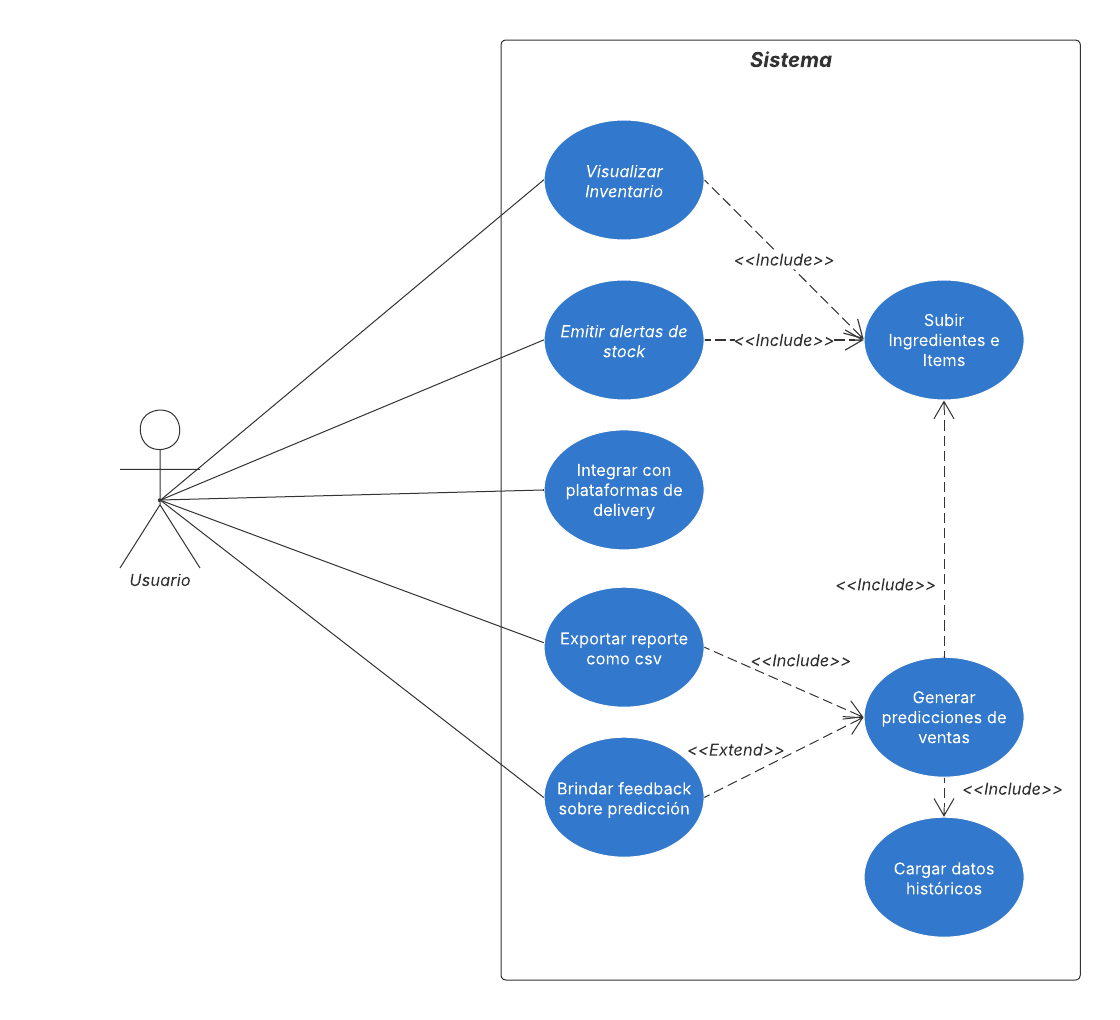
\includegraphics[width=0.7\textwidth]{images/DiagramaCasosDeUsoTesis.png}
    \caption{Diagrama de Casos de Uso}
    \label{fig:casos-de-uso}
\end{figure}

\subsection{Diagramas de Flujo}\label{sec:diagramas-flujo}

Los diagramas de flujo o de procesos son herramientas visuales que representan de manera secuencial los pasos y decisiones que conforman un procedimiento. Su utilización permite clarificar la lógica del negocio, identificar posibles ineficiencias y redundancias, así como facilitar la comunicación entre los equipos técnicos y los usuarios. De esta manera, constituyen un recurso fundamental para comprender, analizar, documentar y mejorar procesos organizacionales \parencite{asq2025flowchart}.

\subsubsection{Registro y Autenticación}

Con el fin de garantizar la seguridad y la personalización de los datos, el acceso a la información y a las funcionalidades críticas de SmartStocker se encuentra restringido a usuarios autenticados. Para ello, la plataforma implementa un flujo de registro inicial y un mecanismo de inicio de sesión que permite identificar de manera única a cada restaurante o local gastronómico.

En la etapa de registro, el usuario debe proporcionar credenciales seguras junto con los datos básicos de su establecimiento. Una vez verificados y almacenados en la base de datos, se habilita la creación de una cuenta que asegura un entorno exclusivo para la gestión de inventario y el análisis de ventas.

\begin{figure}[htbp]
    \centering
    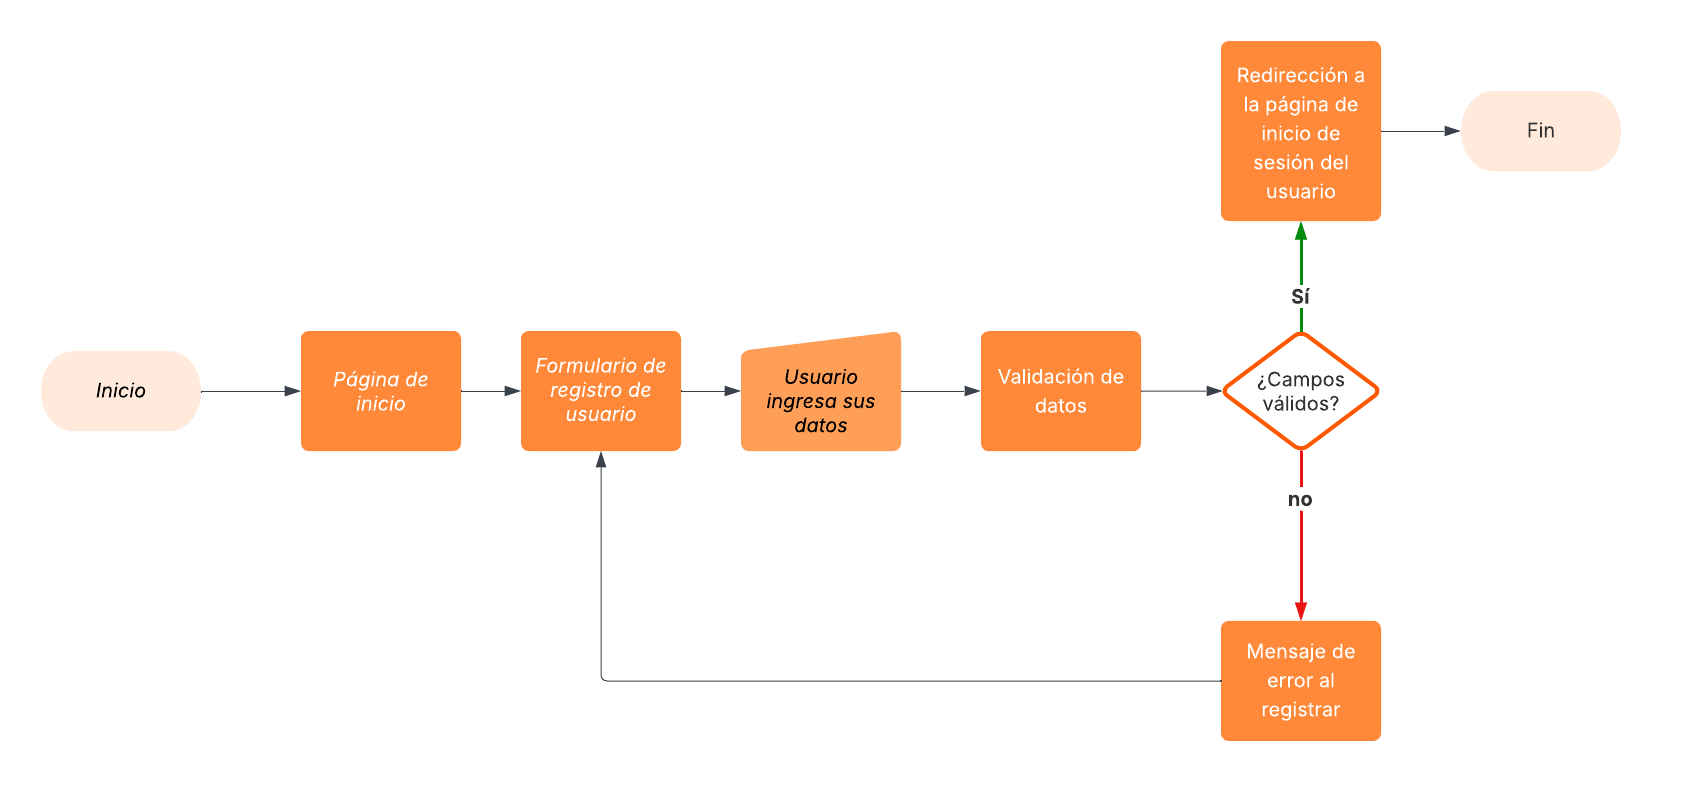
\includegraphics[width=0.7\textwidth]{images/DiagramaRegistroDeUsuario.png}
    \caption{Flujo de Registro del Usuario}
    \label{fig:flujo-registro}
\end{figure}

Posteriormente, mediante la autenticación, los usuarios acceden a su espacio de trabajo personalizado, desde el cual es posible consultar métricas, visualizar predicciones de demanda, administrar productos e ingredientes y recibir alertas relacionadas con el stock disponible. Este proceso de inicio de sesión no solo protege la integridad de la información, sino que también garantiza que las recomendaciones generadas por el sistema respondan a las características particulares de cada negocio gastronómico.

\begin{figure}[htbp]
    \centering
    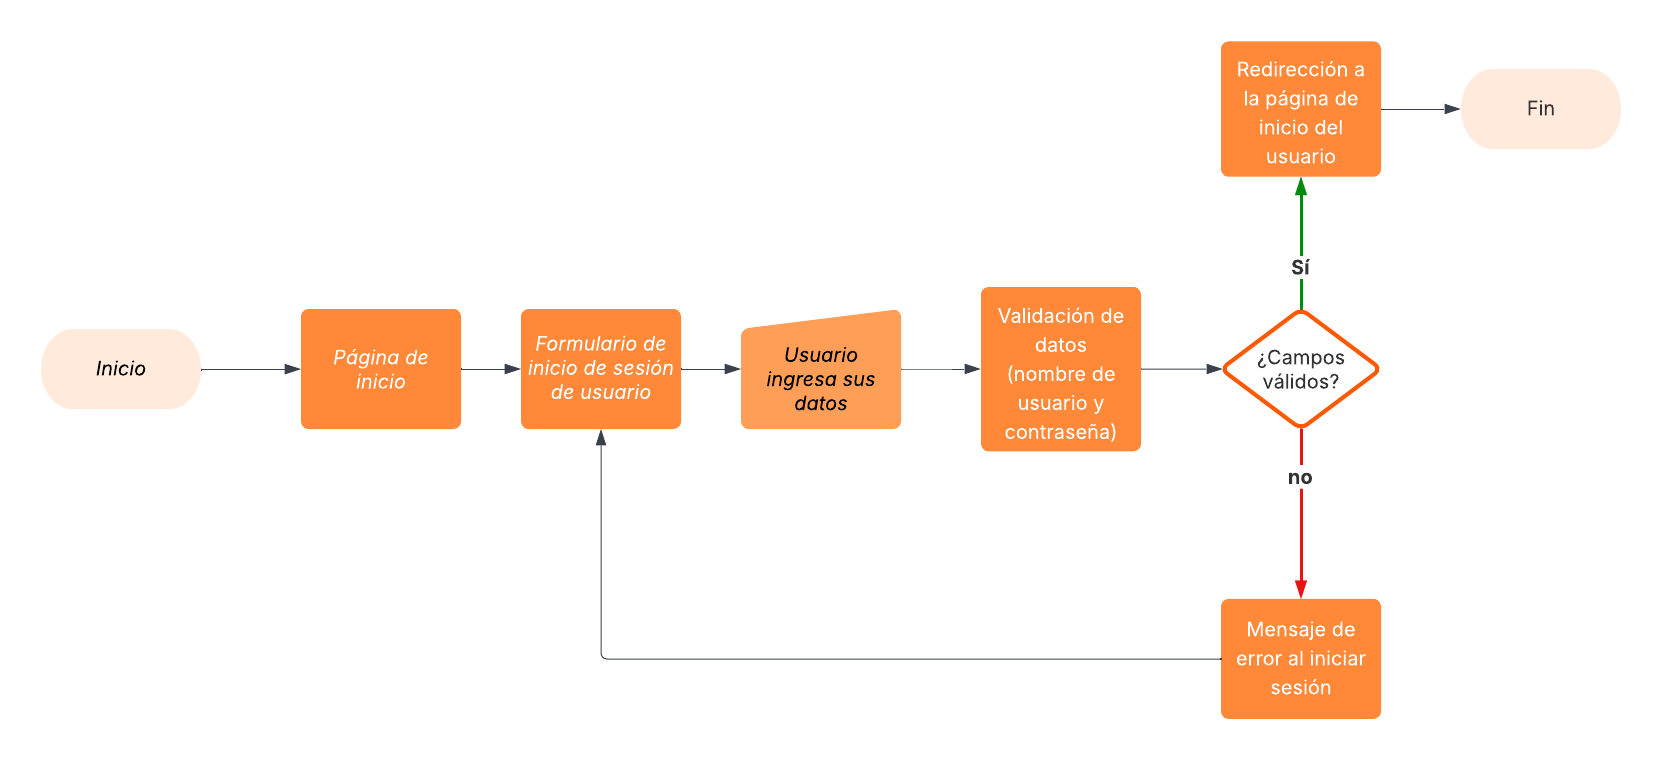
\includegraphics[width=0.7\textwidth]{images/DiagramaInicioDeSesion.png}
    \caption{Flujo de Autenticación del Usuario}
    \label{fig:flujo-autenticacion}
\end{figure}

\subsubsection{Generación de Predicciones}

La capacidad de anticipar la demanda de productos constituye la funcionalidad central de SmartStocker, ya que permite a los restaurantes y locales gastronómicos tomar decisiones fundamentadas sobre compras y reposiciones de insumos. En este proceso, el sistema aplica modelos de Machine Learning que, a partir de datos históricos y variables externas, generan estimaciones confiables de ventas futuras.
\begin{figure}[htbp]
    \centering
    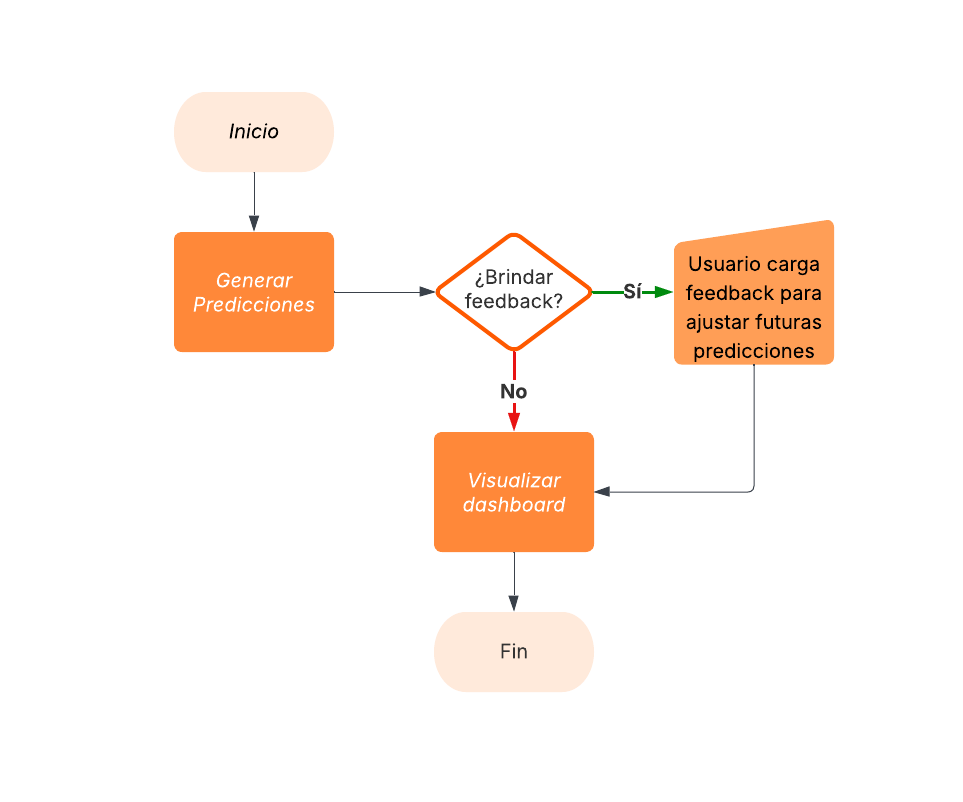
\includegraphics[width=0.7\textwidth]{images/DiagramaDePrediccionTesis.png}
    \caption{Flujo de Predicción de Ventas}
    \label{fig:flujo-prediccion}
\end{figure}

\section{Diseño UX / UI}

El diseño visual de SmartStocker se sustenta en una paleta cromática la cual fue escogida con el propósito de transmitir profesionalismo, confianza y modernidad, atributos que resultan esenciales en un sistema orientado a la toma de decisiones estratégicas en el sector gastronómico. Ahora bien, la elección de los tonos se realizó considerando tanto la dimensión estética como la funcionalidad comunicativa de cada color dentro de la interfaz.

Los colores principales corresponden a una gama de azules, donde el azul corporativo (\#1E40AF) se utiliza en encabezados, botones primarios y elementos de navegación clave. Este tono se asocia tradicionalmente con la seriedad, la estabilidad y la confianza, lo que refuerza la credibilidad del sistema frente a los usuarios que deben basar sus decisiones en datos precisos. Como complemento, el azul claro (\#3B82F6) aparece en estados de interacción como hover y en componentes secundarios, aportando un contraste visual que mantiene la coherencia cromática y facilita la detección rápida de acciones disponibles.

En cuanto a los colores semánticos, se definieron tres que cumplen un rol fundamental en la comunicación de estados del sistema: verde éxito (\#10B981), naranja advertencia (\#F59E0B) y rojo crítico (\#EF4444). Estos colores no solo cumplen con la convención culturalmente reconocida (verde como positivo, rojo como error), sino que también permiten que el usuario identifique de forma inmediata la condición de un insumo o la validez de una acción.

Los colores de apoyo, grises en diferentes intensidades y blanco como fondo principal, cumplen la función de dar equilibrio visual. El gris oscuro (\#1F2937) se emplea en textos principales para asegurar legibilidad, mientras que el gris medio (\#6B7280) se reserva para información secundaria, evitando así la sobrecarga cognitiva. Además, el gris claro (\#F3F4F6) y el azul muy claro (\#EFF6FF) sirven como fondos sutiles y separadores, permitiendo estructurar la información en bloques diferenciados sin necesidad de líneas divisorias excesivas.

En conjunto, esta paleta de colores no responde únicamente a una intención estética, sino que está al servicio de la usabilidad, la accesibilidad y la experiencia de usuario. Cada tonalidad se integra en un sistema visual coherente que facilita la navegación, refuerza el reconocimiento de patrones y garantiza que los usuarios puedan interactuar con la plataforma de forma intuitiva y eficiente.

\begin{table}[htbp]
    \centering
    \begin{tabular}{|l|c|c|}
        \hline
        \textbf{Categoría} & \textbf{Color} & \textbf{Código Hex} \\ \hline
        Azul corporativo & \cellcolor[HTML]{1E40AF} & \#1E40AF \\ \hline
        Azul claro & \cellcolor[HTML]{3B82F6} & \#3B82F6 \\ \hline
        Verde éxito & \cellcolor[HTML]{10B981} & \#10B981 \\ \hline
        Naranja advertencia & \cellcolor[HTML]{F59E0B} & \#F59E0B \\ \hline
        Rojo crítico & \cellcolor[HTML]{EF4444} & \#EF4444 \\ \hline
        Gris oscuro (texto principal) & \cellcolor[HTML]{1F2937} & \#1F2937 \\ \hline
        Gris medio (texto secundario) & \cellcolor[HTML]{6B7280} & \#6B7280 \\ \hline
        Gris claro (fondos) & \cellcolor[HTML]{F3F4F6} & \#F3F4F6 \\ \hline
        Azul muy claro (fondos) & \cellcolor[HTML]{EFF6FF} & \#EFF6FF \\ \hline
    \end{tabular}
    \caption{Paleta de colores empleada en SmartStocker}
    \label{tab:paleta-colores}
\end{table}

\section{Pantallas de la aplicación}

A continuación, se presentan las principales pantallas de la aplicación SmartStocker, organizadas según el flujo de interacción del usuario. Estas capturas ilustran tanto la experiencia inicial (Figura~\ref{fig:ux-landing1} a \ref{fig:ux-landing5})  como la gestión de datos (Figura~\ref{fig:ux-ingredientes} a Figura~\ref{fig:ux-nuevo-ingrediente}) y las funcionalidades clave de predicción de ventas (Figura~\ref{fig:ux-predicciones} a Figura~\ref{fig:ux-prediccion2}).

\begin{figure}[htbp]
    \centering
    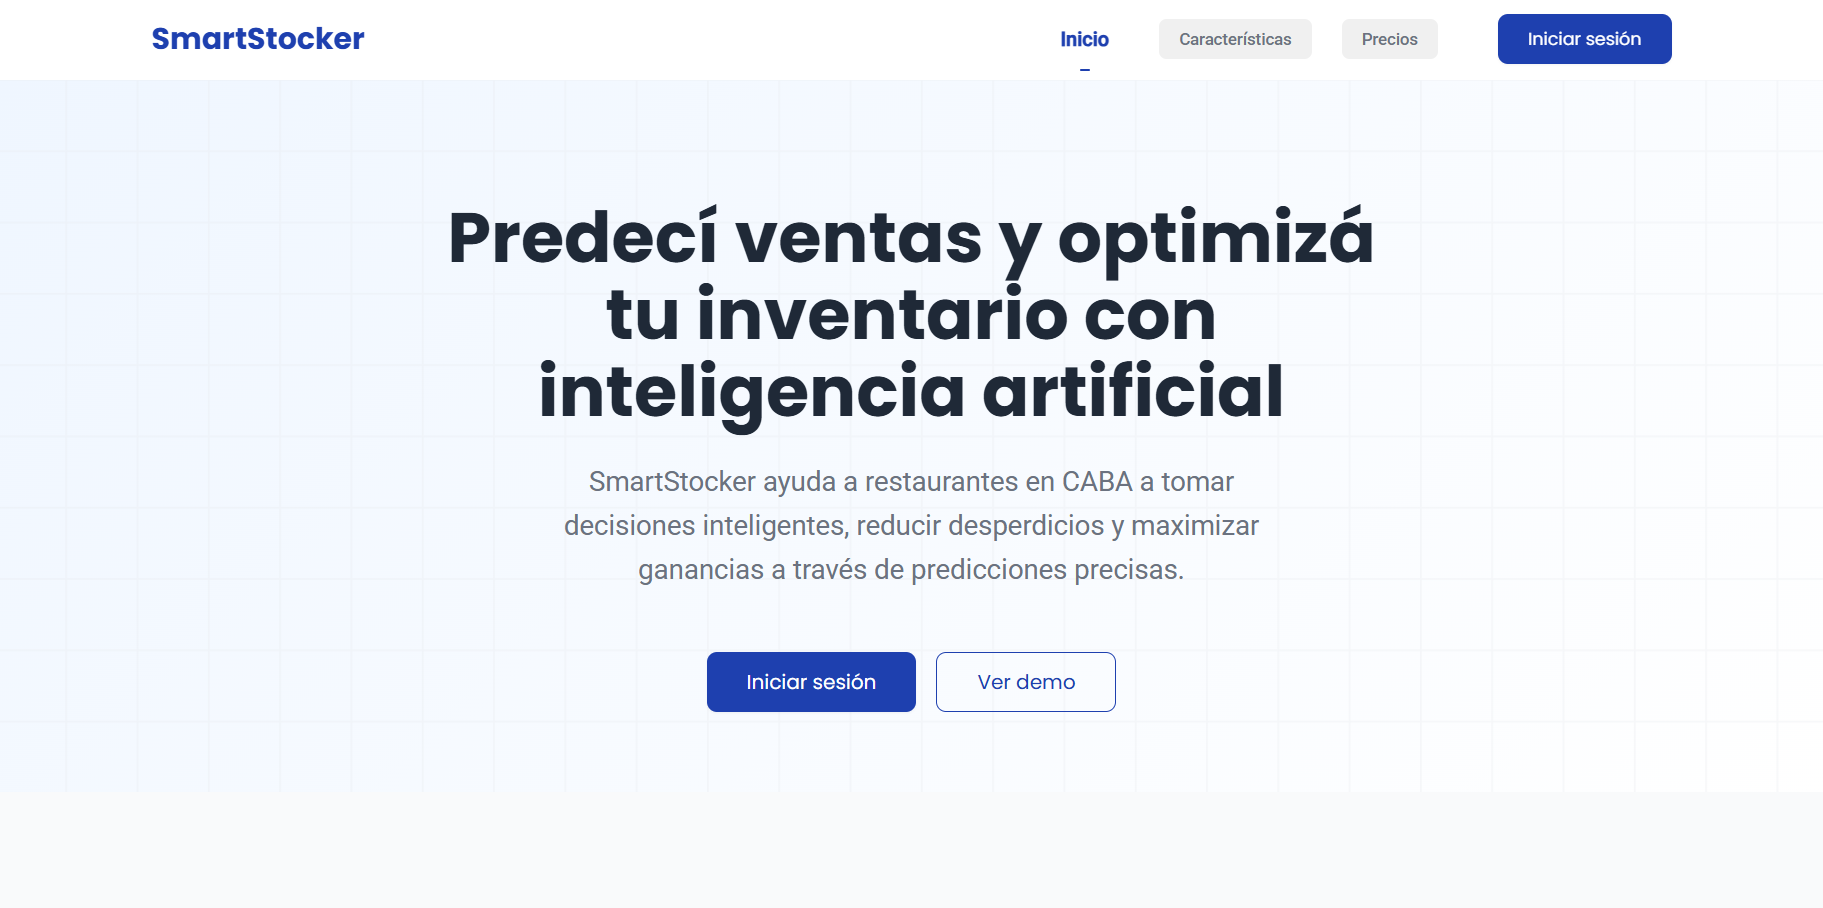
\includegraphics[width=0.9\textwidth]{images/landing1.png}
    \caption{Pantalla de inicio (Landing) – Parte 1}
    \label{fig:ux-landing1}
\end{figure}

\begin{figure}[htbp]
    \centering
    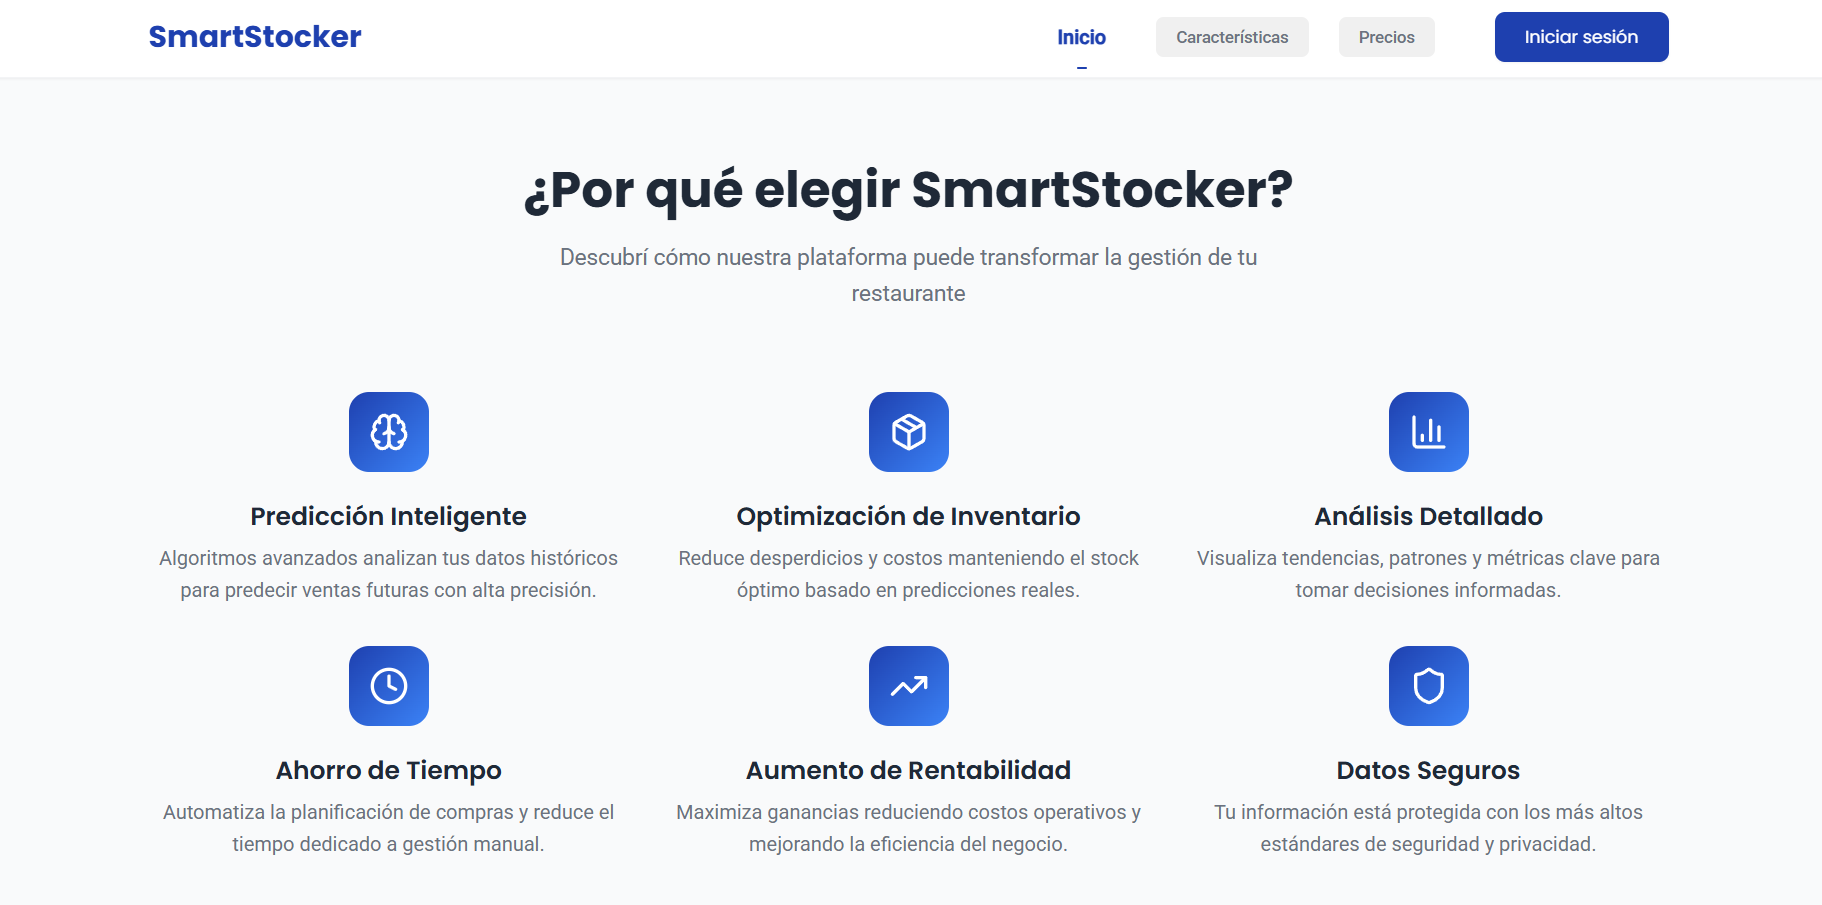
\includegraphics[width=0.9\textwidth]{images/landing2.png}
    \caption{Pantalla de inicio (Landing) – Parte 2}
    \label{fig:ux-landing2}
\end{figure}

\begin{figure}[htbp]
    \centering
    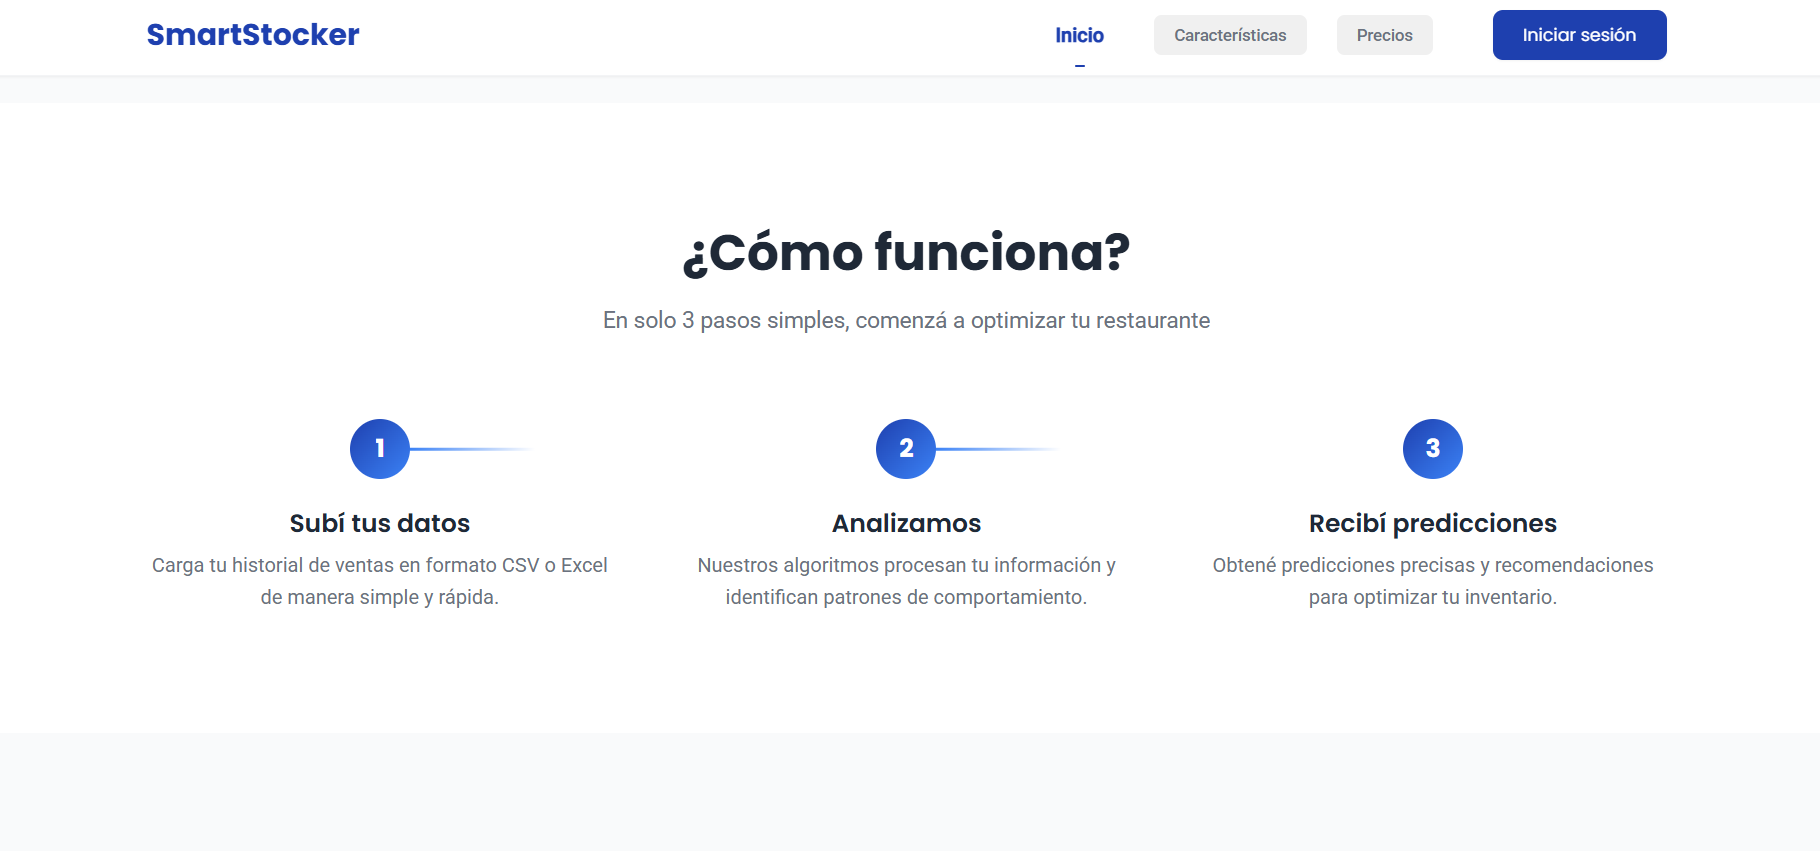
\includegraphics[width=0.9\textwidth]{images/landing3.png}
    \caption{Pantalla de inicio (Landing) – Parte 3}
    \label{fig:ux-landing3}
\end{figure}

\begin{figure}[htbp]
    \centering
    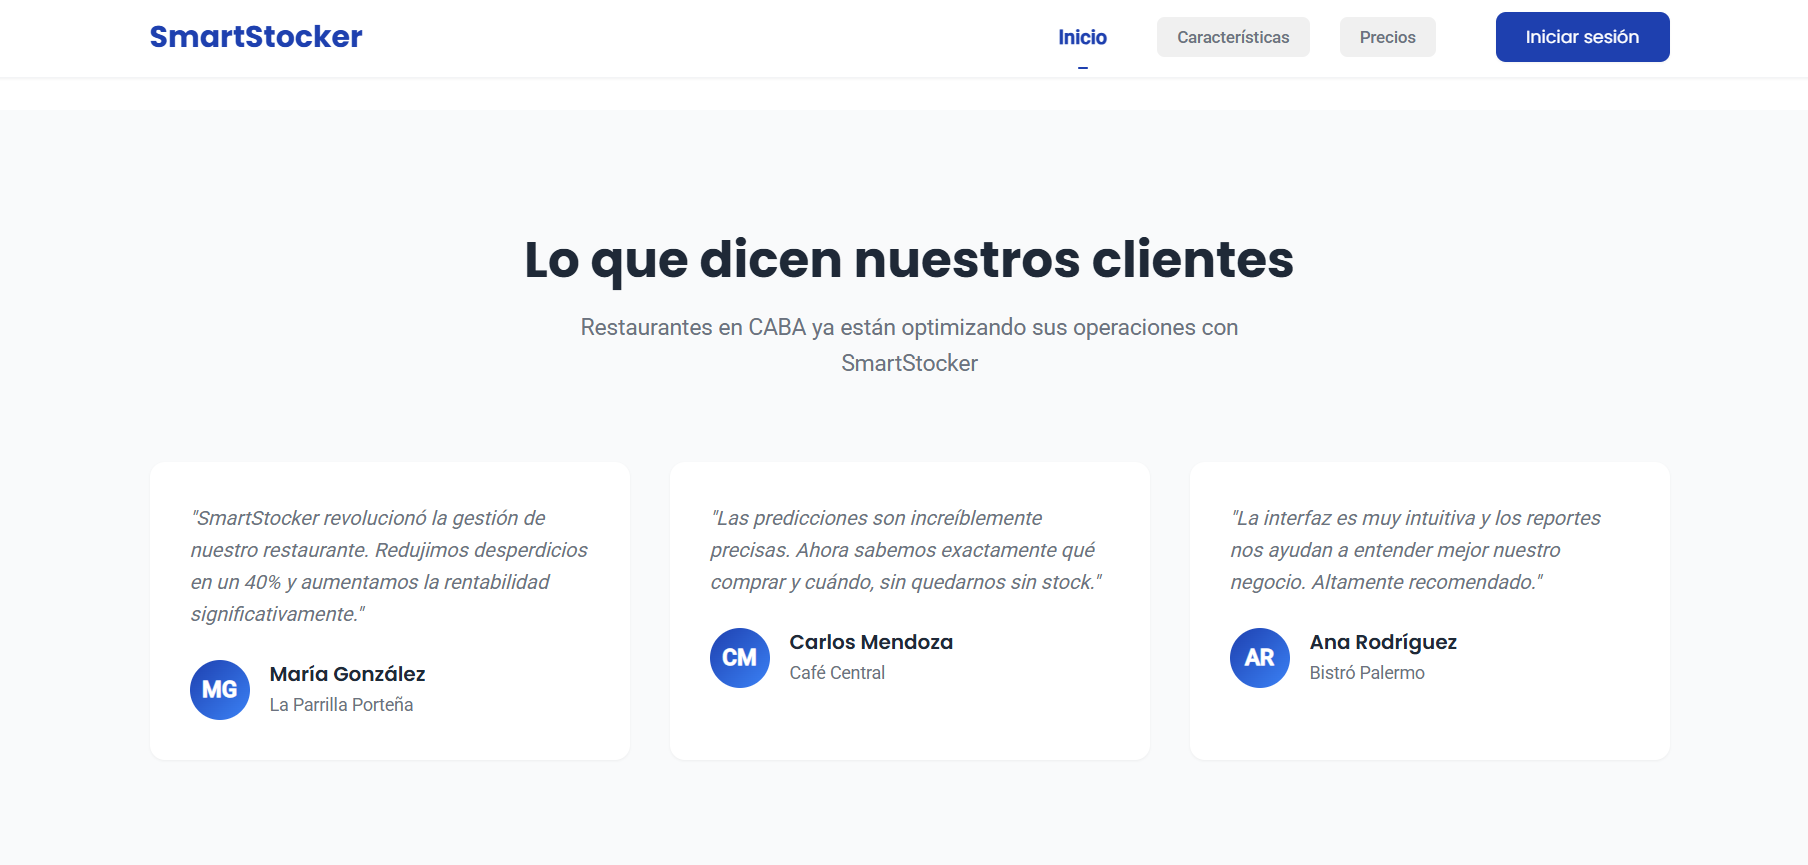
\includegraphics[width=0.9\textwidth]{images/landing4.png}
    \caption{Pantalla de inicio (Landing) – Parte 4}
    \label{fig:ux-landing4}
\end{figure}

\begin{figure}[htbp]
    \centering
    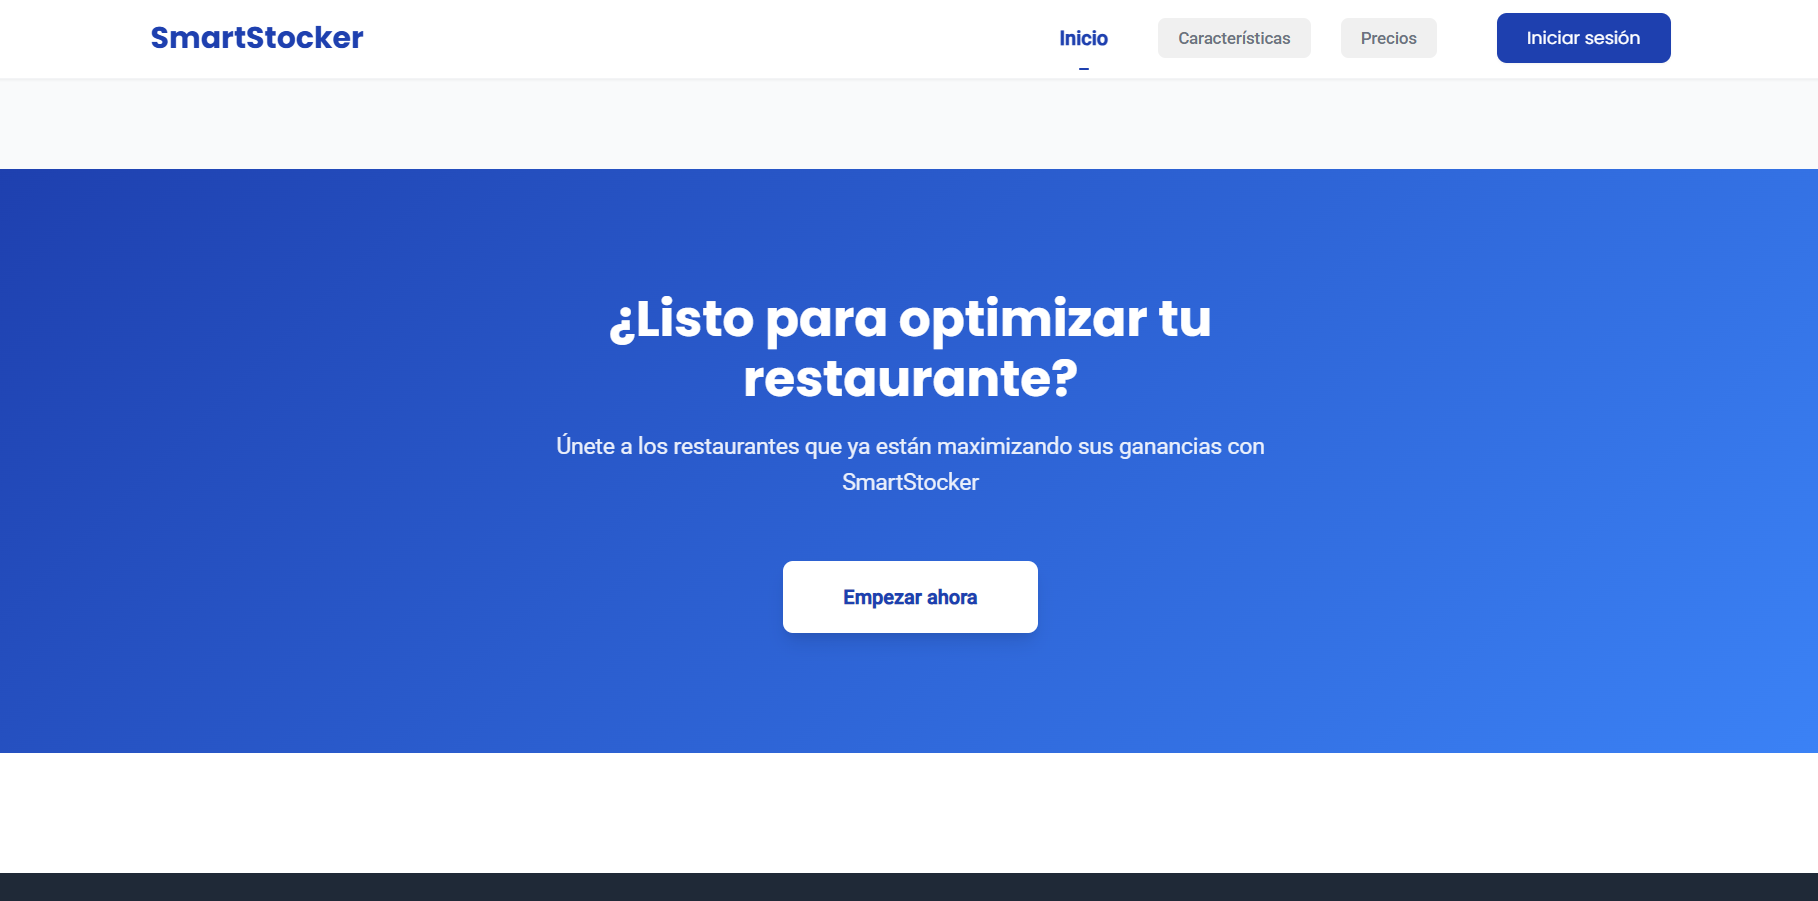
\includegraphics[width=0.9\textwidth]{images/landing5.png}
    \caption{Pantalla de inicio (Landing) – Parte 5}
    \label{fig:ux-landing5}
\end{figure}

\begin{figure}[htbp]
    \centering
    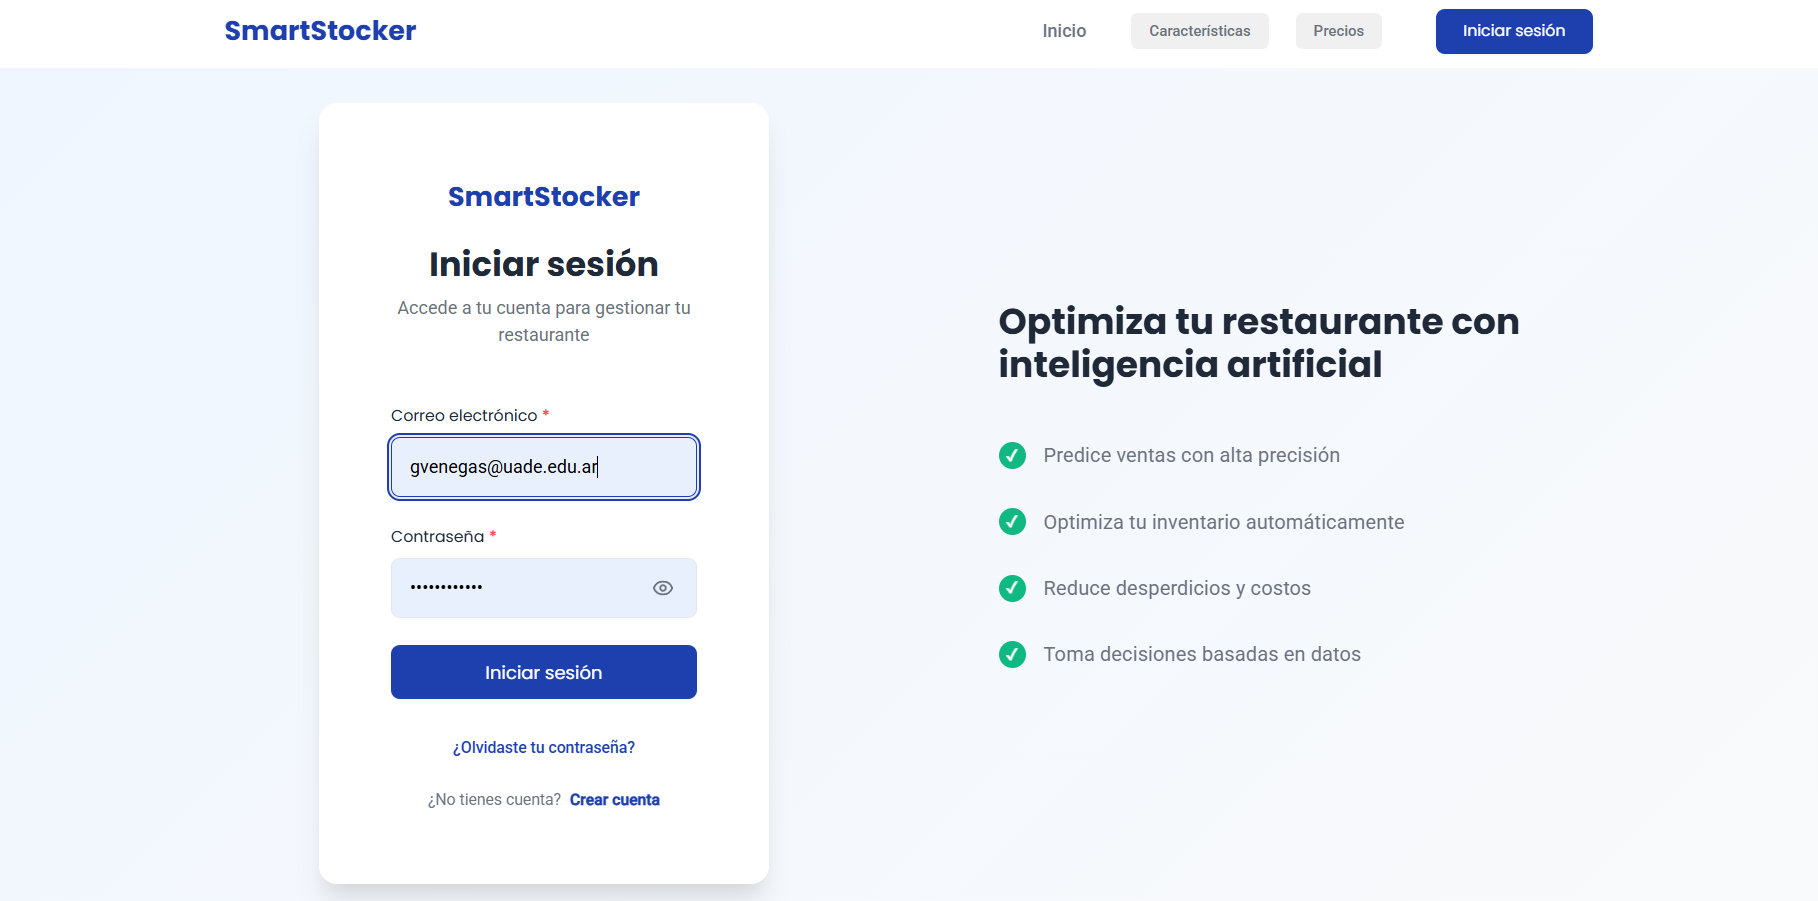
\includegraphics[width=0.9\textwidth]{images/login.png}
    \caption{Pantalla de inicio de sesión}
    \label{fig:ux-login}
\end{figure}

\begin{figure}[htbp]
    \centering
    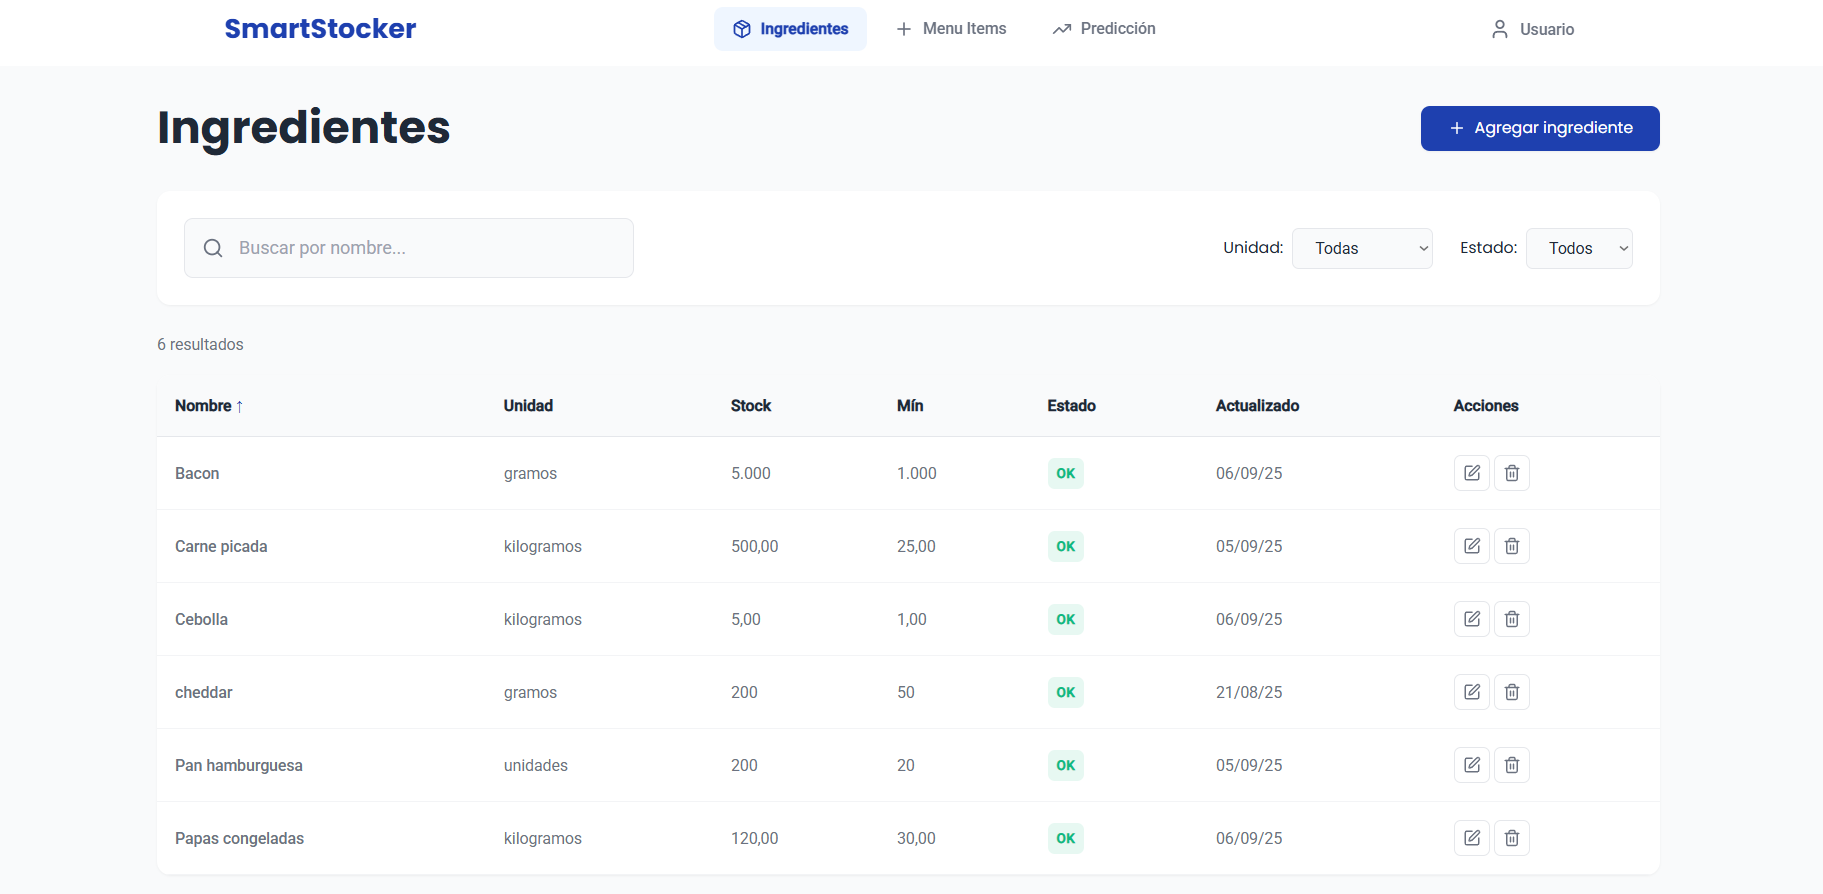
\includegraphics[width=0.9\textwidth]{images/ingredientes.png}
    \caption{Pantalla de gestión de ingredientes}
    \label{fig:ux-ingredientes}
\end{figure}

\begin{figure}[htbp]
    \centering
    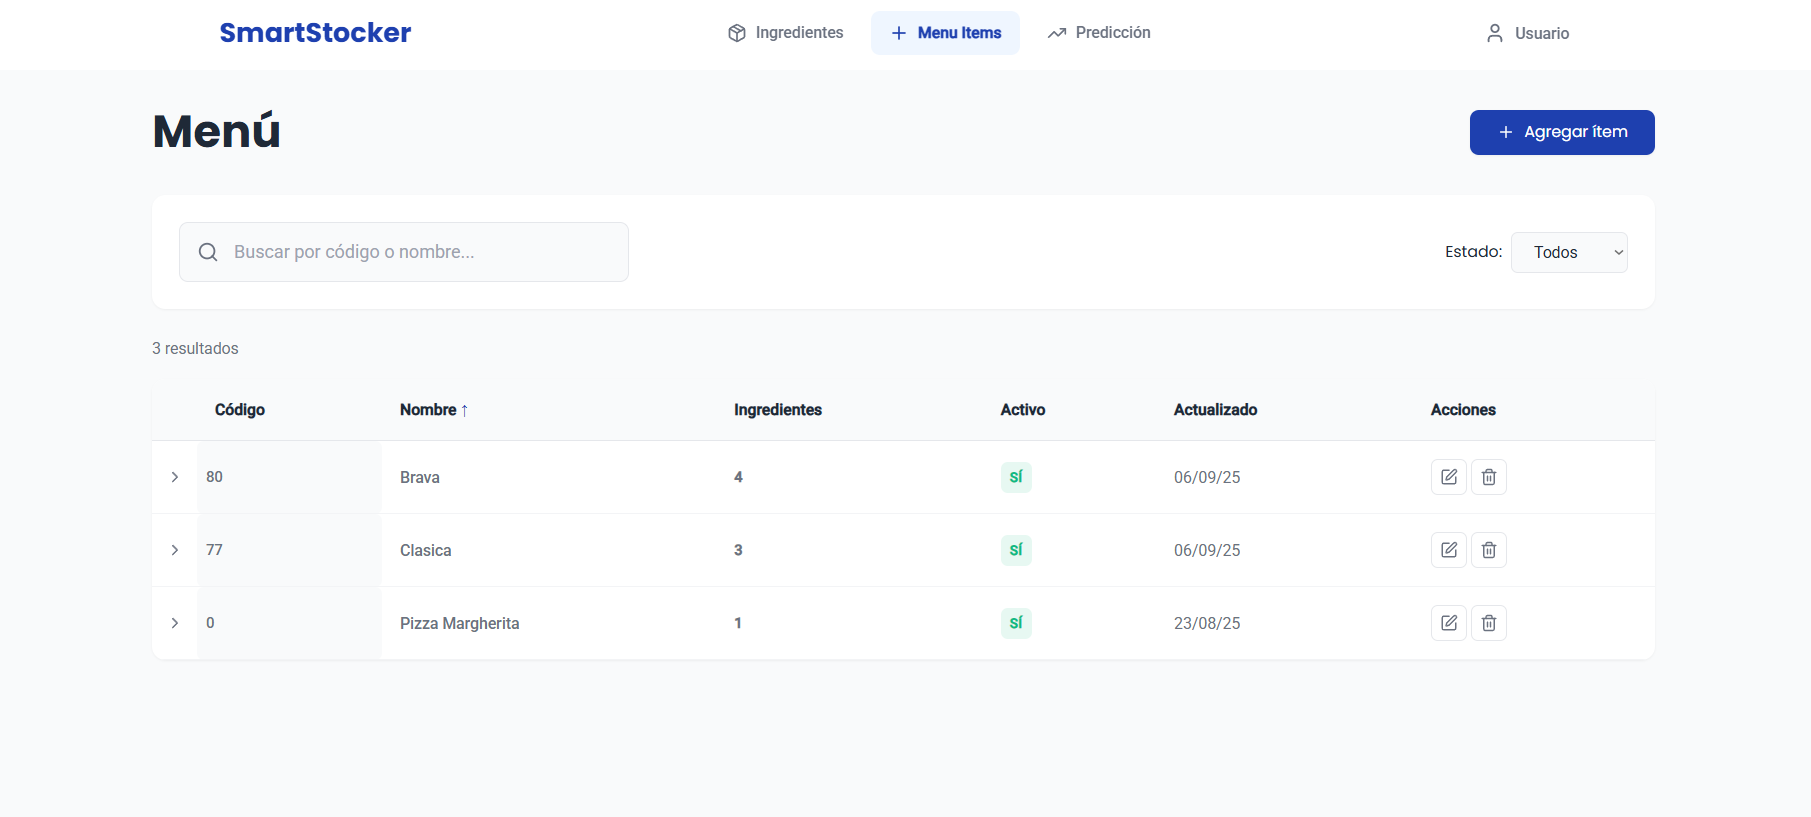
\includegraphics[width=0.9\textwidth]{images/items.png}
    \caption{Pantalla de gestión de ítems}
    \label{fig:ux-items}
\end{figure}

\begin{figure}[htbp]
    \centering
    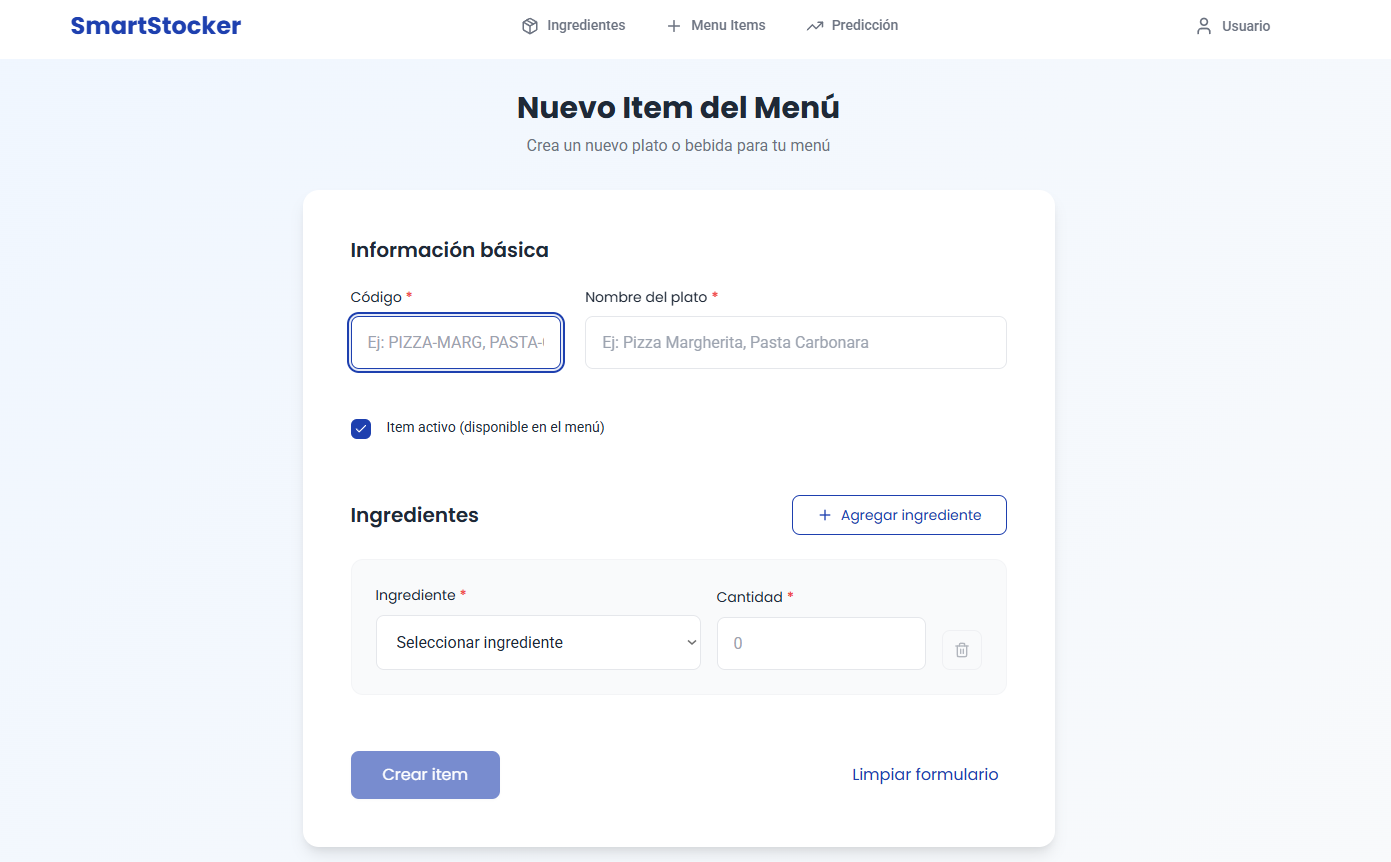
\includegraphics[width=0.9\textwidth]{images/nuevoItem.png}
    \caption{Pantalla para agregar un nuevo ítem}
    \label{fig:ux-nuevo-item}
\end{figure}

\begin{figure}[htbp]
    \centering
    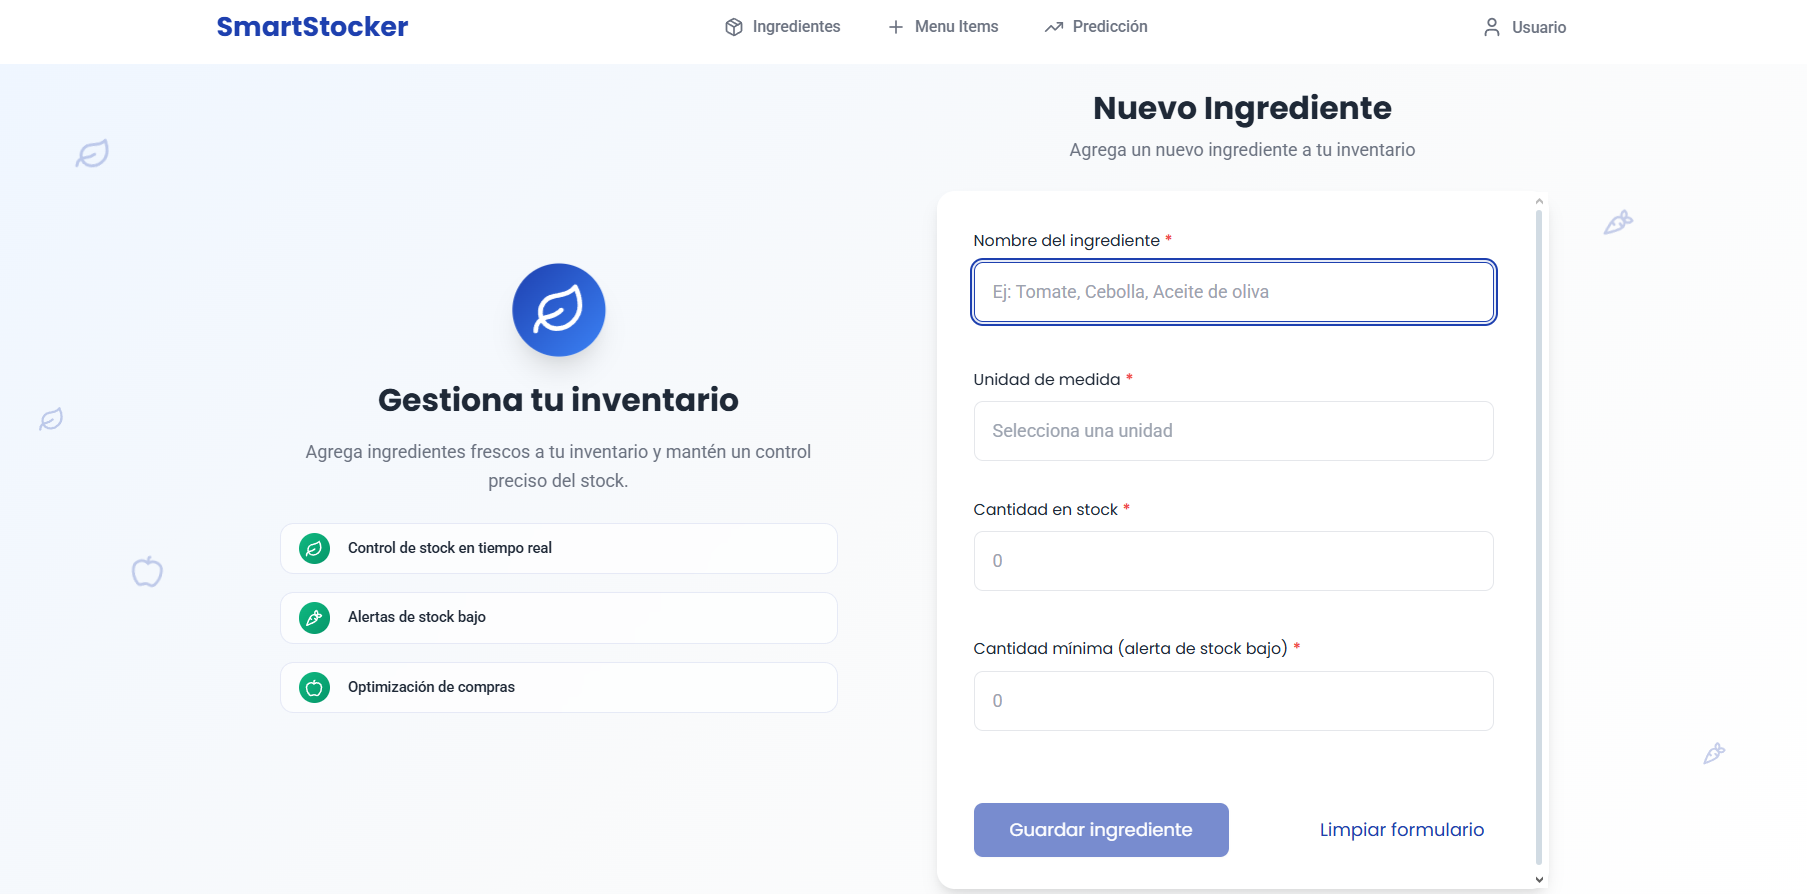
\includegraphics[width=0.9\textwidth]{images/nuevoIngrediente.png}
    \caption{Pantalla para agregar un nuevo ingrediente}
    \label{fig:ux-nuevo-ingrediente}
\end{figure}

\begin{figure}[htbp]
    \centering
    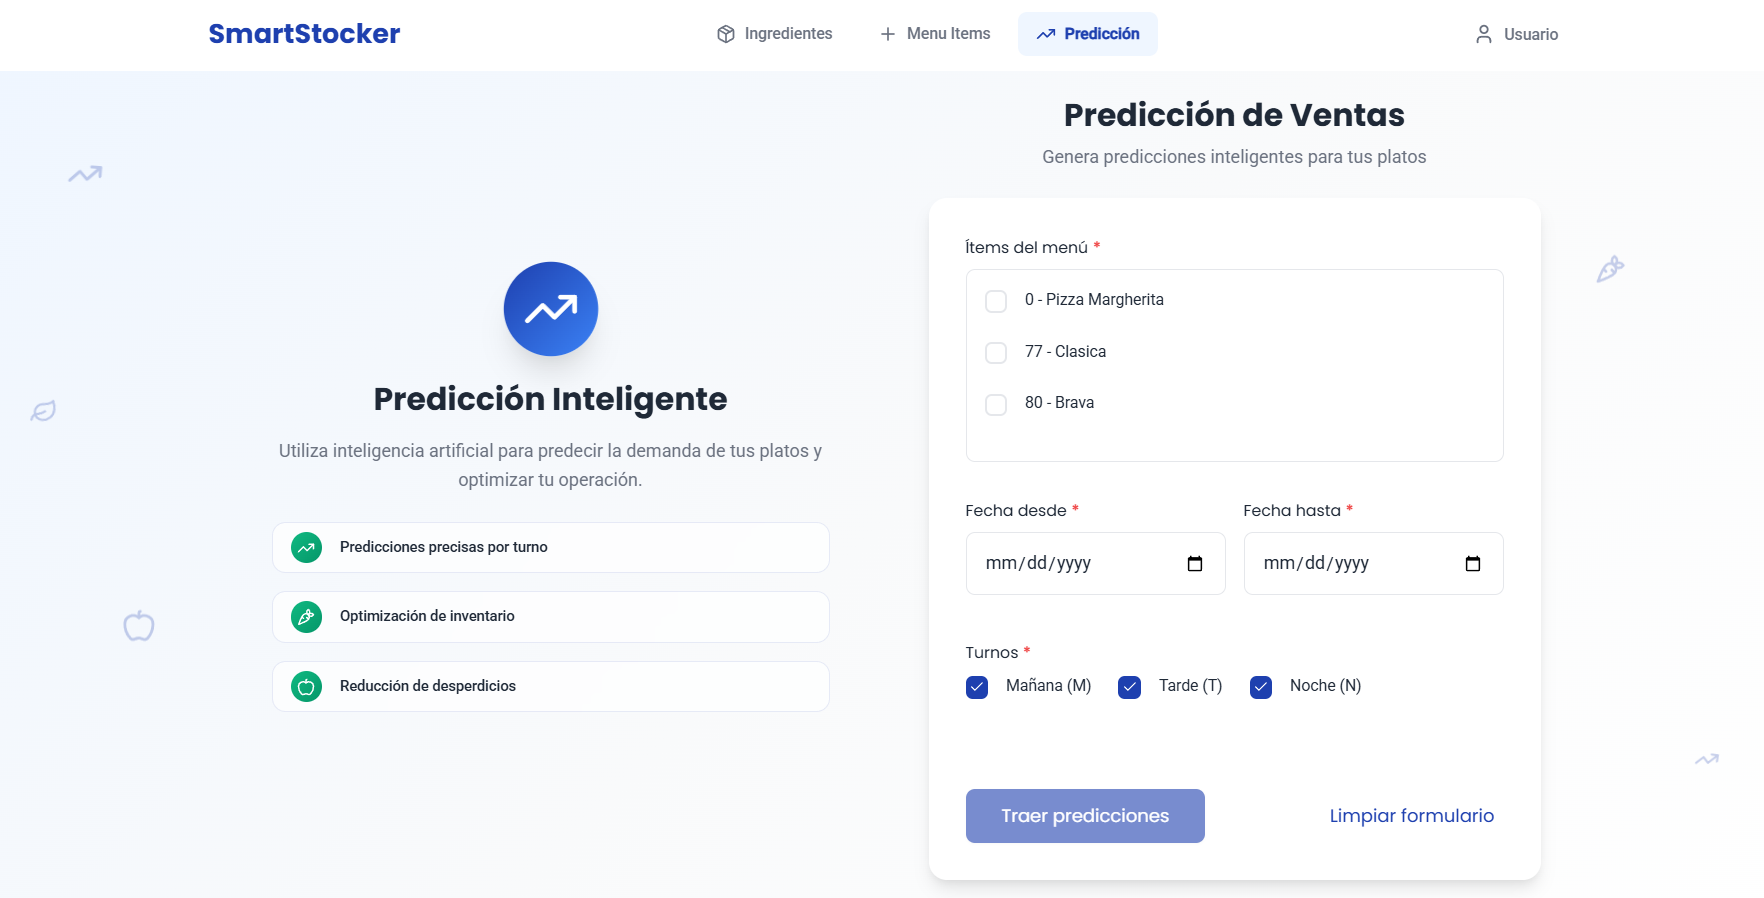
\includegraphics[width=0.9\textwidth]{images/predicciones.png}
    \caption{Pantalla consolidada de predicciones}
    \label{fig:ux-predicciones}
\end{figure}

\begin{figure}[htbp]
    \centering
    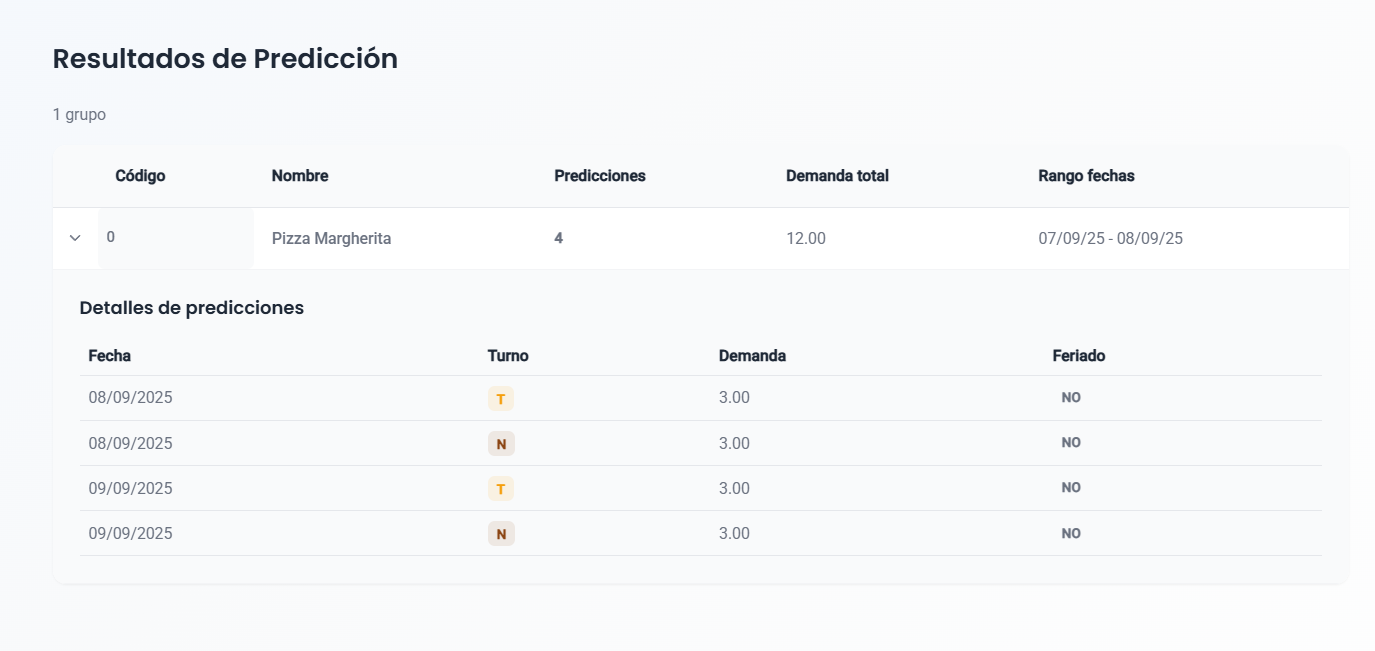
\includegraphics[width=0.9\textwidth]{images/prediccion1.png}
    \caption{Resultado de predicciones}
    \label{fig:ux-prediccion1}
\end{figure}

\begin{figure}[htbp]
    \centering
    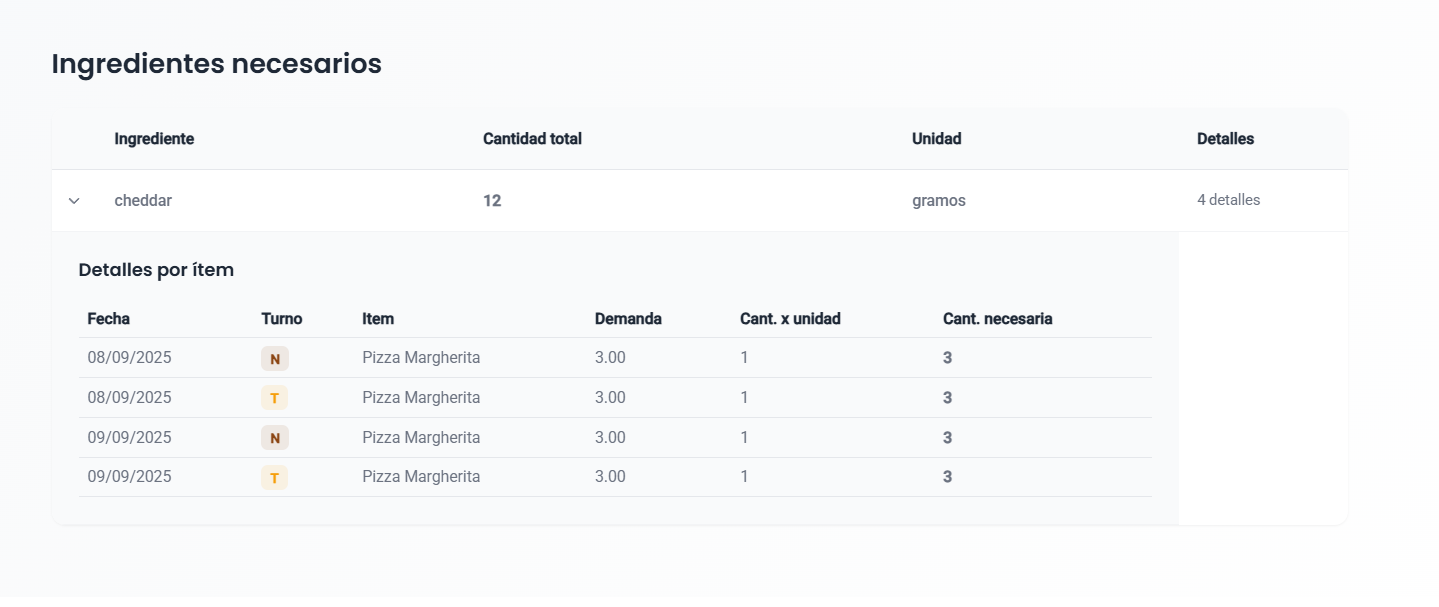
\includegraphics[width=0.9\textwidth]{images/prediccion2.png}
    \caption{Ingredientes necesarios}
    \label{fig:ux-prediccion2}
\end{figure}

\section{Funcionalidades}\label{sec:funcionalidades}

\subsection{Predicción de Ventas}\label{sec:prediccion-ventas}

En el sector gastronómico, la capacidad de anticipar la demanda se ha convertido en un factor estratégico para reducir pérdidas, optimizar el uso de insumos y garantizar la continuidad del servicio. Bajo dicha premisa, SmartStocker incorpora un módulo de predicciones como una de sus funcionalidades principales. El sistema aplica técnicas de aprendizaje automático que permiten transformar datos históricos y registros actuales en estimaciones de ventas futuras. 

El objetivo de esta funcionalidad es reemplazar las decisiones basadas únicamente en la experiencia o la intuición por un enfoque sistemático apoyado en datos, incrementando la objetividad en la gestión del inventario. Además, su integración con fuentes externas de información le otorga la capacidad de adaptarse a contextos cambiantes, como la estacionalidad, los feriados o incluso factores climáticos que pueden influir en el consumo.

\subsection{Fuentes de Datos}\label{sec:fuentes-datos}

El modelo predictivo requiere datos de calidad para generar resultados confiables. Con este fin, la plataforma web admite dos vías principales de recopilación:

\begin{itemize}
    \item \textbf{Carga manual de datos mediante archivos CSV}: esta modalidad permite a los locales gastronómicos incorporar sus registros históricos directamente desde sistemas internos o planillas de control. Para este fin, se determinó que el formato esperado para archivos CSV es:
    \begin{itemize}
        \item Fecha venta: dd/mm/aaaa hh:mm:ss
        \item Producto: con el mismo nombre usado al generar el producto en la aplicación.
        \item Cantidad.
    \end{itemize}

    \item \textbf{Integración automática con sistemas de venta}: este mecanismo posibilita la importación continua de pedidos en tiempo real desde aplicaciones como PedidosYa. Con ello, el sistema asegura la actualización permanente del conjunto de datos, reduciendo la dependencia exclusiva de registros históricos y adaptándose a la dinámica diaria del negocio.
\end{itemize}

\subsection{Gestion de ingredientes e items del menu}\label{sec:carga-datos}

Para que el sistema pueda calcular el inventario sugerido, es necesario que el usuario cargue los ingredientes que utiliza en su local y los vincule con los productos gastronómicos que ofrece en su menú. Esta funcionalidad permite al usuario definir y administrar tanto los ingredientes como los items del menu, permitiendo, en el caso particular de los ingredientes, realizar esta carga no solo desde la UI, sino tambien de forma masiva a traves de un archivo, a fin de simplificar la operatoria en caso de que el usuario cuente con un listado extenso.

\subsection{Procesamiento Predictivo}\label{sec:procesamiento-predictivo}

El procesamiento predictivo constituye el núcleo técnico de la funcionalidad de SmartStocker. Una vez recopilados los datos históricos y actuales, el sistema los somete a un proceso de depuración y normalización que asegura la consistencia y homogeneidad de los registros. Este preprocesamiento incluye la eliminación de valores atípicos, la imputación de datos faltantes y la transformación de variables temporales (como la estacionalidad o los turnos horarios) en características relevantes para el modelo.

Posteriormente, los datos son utilizados para entrenar algoritmos de aprendizaje supervisado, dentro de los cuales se evaluaron diferentes enfoques, priorizando modelos de regresión y técnicas de boosting como CatBoost, debido a su robustez en contextos con variables categóricas y a su capacidad de reducir el sobreajuste. Estos modelos generan proyecciones de ventas futuras en base a patrones identificados, incorporando tanto las tendencias históricas como variables externas tales como clima, feriados y días de la semana.

Las predicciones se ejecutan bajo demanda, es decir, cada vez que el usuario lo requiera dentro de la plataforma, lo que garantiza resultados actualizados y adaptados al contexto puntual de planificación del negocio, integrando un mecanismo de retroalimentación continua (feedback loop) mediante el cual los usuarios validan si las estimaciones reflejaron la demanda real observada; esa información se reintegra al modelo para ajustar progresivamente su precisión, personalizando las predicciones al contexto específico de cada restaurante y favoreciendo la evolución de SmartStocker ante escenarios cambiantes.

En consecuencia, el procesamiento predictivo de SmartStocker no se limita a entregar un valor numérico de ventas estimadas, sino que constituye un sistema adaptable y evolutivo, orientado a respaldar la toma de decisiones estratégicas en la gestión de inventarios gastronómicos.

\subsection{Cálculo de Inventario Sugerido}\label{sec:calculo-inventario}

Una vez obtenidas las predicciones de ventas, los resultados obtenidos son vinculados con la lista de ingredientes definida por el restaurante. De esta manera, se genera un cálculo automático del inventario recomendado, minimizando tanto los riesgos de desabastecimiento como los costos derivados de un exceso de stock. 

\subsection{Notificación de Alertas}\label{sec:alertas}

El módulo de notificaciones cumple un rol preventivo. Cada vez que un insumo alcanza un nivel inferior al umbral configurado por el usuario, el sistema genera una alerta en el tablero principal y, en futuras versiones, podrá enviarlas vía correo electrónico o notificaciones push.

El valor de este componente radica en su capacidad para evitar interrupciones operativas. En un negocio gastronómico, la ausencia de un ingrediente clave no solo afecta la venta de un plato específico, sino que también impacta en la experiencia del cliente y en la reputación del local. Por esta razón, las alertas de stock bajo no deben considerarse únicamente como un aviso técnico, sino como un mecanismo de aseguramiento de la calidad del servicio.


\section{Arquitectura de la solución}\label{sec:arquitectura-solucion}
En esta sección se presenta la arquitectura de SmartStocker, detallando las tecnologías empleadas para su diseño técnico y funcional. La arquitectura funciona como marco conceptual que sustenta cada componente del sistema y especifica las interacciones y dependencias entre las distintas partes que lo componen.

\subsection{Diagrama de Arquitectura conceptual}\label{sec:arquitectura-conceptual}
En relación con la arquitectura de alto nivel de SmartStocker, se propone un modelo de tres capas que organiza la solución, asegurando una separación clara de responsabilidades y mejorando la escalabilidad. Esta estructura está diseñada para optimizar tanto la interacción con el usuario como el procesamiento y almacenamiento de los registros de venta y los resultados de inferencia generados por los modelos predictivos.

La primera capa —Capa de Presentación (Presentation Layer)— agrupa la interfaz y la experiencia de usuario. En ella se implementa el frontend de SmartStocker con Next.js y se despliega mediante AWS Amplify, aprovechando sus capacidades de hosting y CI/CD. Esta capa permite a los usuarios interactuar con la plataforma, gestionar sus productos e ingredientes, visualizar recomendaciones y alertas, y realizar operaciones de predicciones de venta de forma responsiva y orientada a la operativa diaria.

La Capa de Negocio (Business Layer) constituye el núcleo lógico de SmartStocker y se organiza en tres componentes principales. El primero es una API REST que actúa como puente entre la capa de presentación y los servicios backend; a través de ella se gestionan las sesiones y la autorización, se exponen los endpoints para solicitar predicciones y gestionar productos, ingredientes, y alertas, y se que incluye la lógica necesaria para atender las demandas de la interfaz de usuario de forma segura y consistente. Esta se encuentra desarollada con Node.js, a fin de aprovechar lo mas posible su integracion nativa con Next.js, y la simpleza a la hora de desplegar la api de forma serverless mediante AWS Lambda. El segundo es el pipeline de ETL, encargado de recibir los datos de ventas en tiempo real desde los sistemas externos, procesarlos, enriquecerlos, y dejarlos listos para ser usados por el modelo. Por último, el pipeline de ML será el encargado de realizar el entrenamiento del modelo, ya sea de forma periódica u on demand, y de dejarlo disponible para su uso en las operaciones de inferencia. La logica de ambos pipelines se encuentra desarollada en Python, a fin de aprovechar las distintas librerías y frameworks disponibles para el procesamiento de datos y machine learning, y se encuentran implementados mediante AWS Lambda.

Por último, la Capa de Almacenamiento (Storage Layer) se organiza según los distintos casos de uso de la plataforma y está diseñada para optimizar rendimiento y costos. Los datos de la aplicación, tales como los ingredientes, productos, ventas realizadas,  y resultados de predicciones, se almacenan en DocumentDB, lo que facilita lecturas de baja latencia y flexibilidad en la estructura de los datos. Mientras tanto, los datos orientados al entrenamiento del modelo, tales como los datasets históricos, los artefactos de entrenamiento y los modelos exportados se almacenan en Amazon S3, aprovechando su durabilidad y su bajo costo.

\begin{figure}[H]
    \centering
    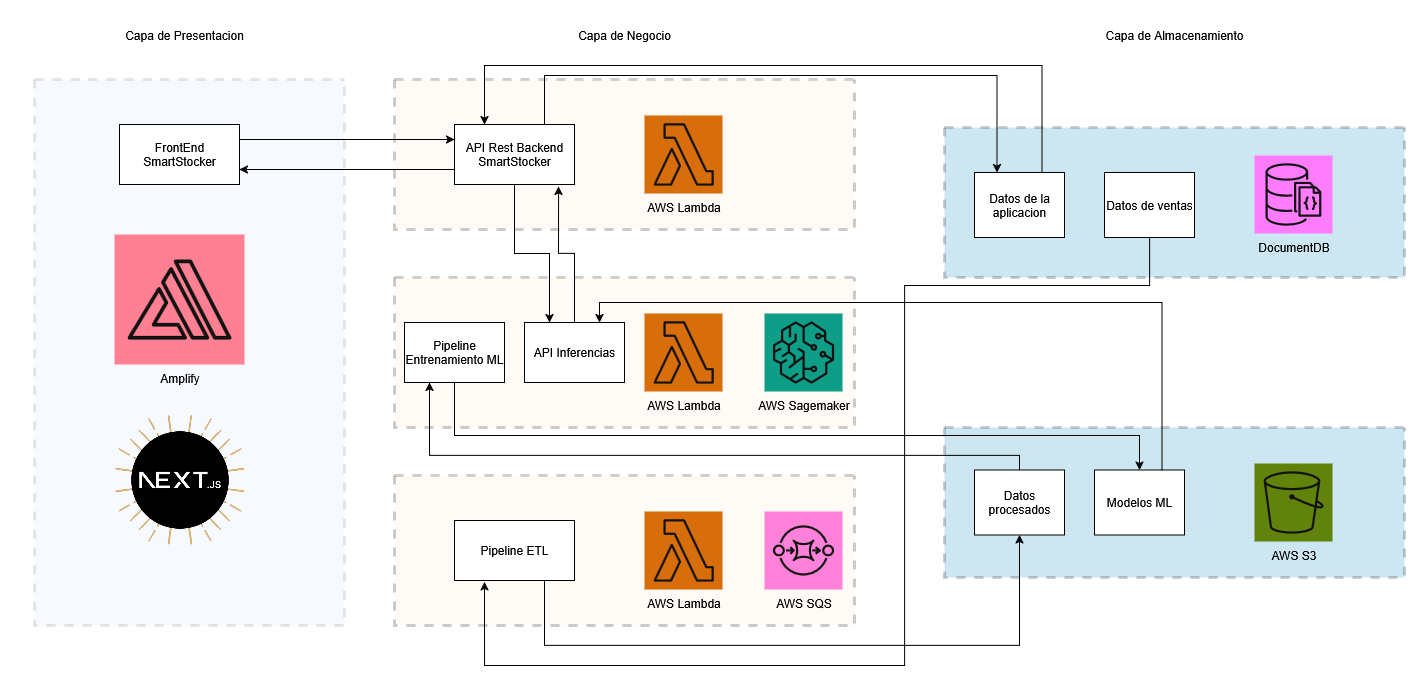
\includegraphics[width=1\textwidth]{images/arquitectura_capas.png}
    \caption{Arquitectura conceptual de SmartStocker}
    \label{fig:arquitectura-conceptual}
\end{figure}

\subsection{Diagrama de Despliegue}\label{sec:arquitectura-despliegue}
Se decidió usar Amazon Web Services (AWS) como solución de despliegue para nuestra solución, debido a la flexibilidad y amplitud de herramientas ofrecidas necesarias para implementar la arquitectura de SmartStocker.

Analizando la capa de presentación, esta se encuentra desarrollada con Next.js, y desplegado a través de AWS Amplify. Se eligió este servicio puesto que simplifica enormemente la gestión de la aplicación, permitiendo, mediante una simple configuración inicial, encargarse de aspectos tales como el despliegue (permitiendo CI/CD integrado a GitHub), hasta del escalamiento en sí.

Para la capa de almacenamiento, se optaron por dos soluciones. Primero, DocumentDB como base de datos NoSQL, seleccionado debido a la naturaleza no estructurada de los datos a utilizar, y que nos brinda la posibilidad de modificar el schema con facilidad, además de ser una base serverless escalable. Y segundo, S3, para contener la información en formato \verb|csv| requerida para los entrenamientos del modelo, y para almacenar los archivos correspondientes al modelo entrenado en si.

Para la capa de negocio, se decidió implementar las distintas APIs requeridas mediante AWS Lambda, dado que su enfoque serverless permite abstraernos de la gestión de la infraestructura, acelerando el desarrollo y la puesta en producción, escalando cuando la demanda lo requiera, y reduciendo los costos fijos.

Esto también aplica para el pipeline de ETL, donde también se utiliza AWS Simple Queue Service (SQS) para desacoplar el procesamiento de las ventas, a fin de lograr velocidades de respuesta rápida ante los sistemas externos que enviaran las mismas, mientras que el procesamiento y enriquecimiento de las ventas se realiza en otra Lambda.

Por último, se decidió usar AWS Sagemaker en el pipeline de ML, puesto que simplifica enormemente el entrenamiento del modelo, requiriendo suministrarle solamente el dataset a utilizar, y permite disponibilizar el modelo para ser usado para predicciones mediante endpoints, lo que brinda una consulta rápida y de fácil implementación.

\begin{figure}[H]
    \centering
    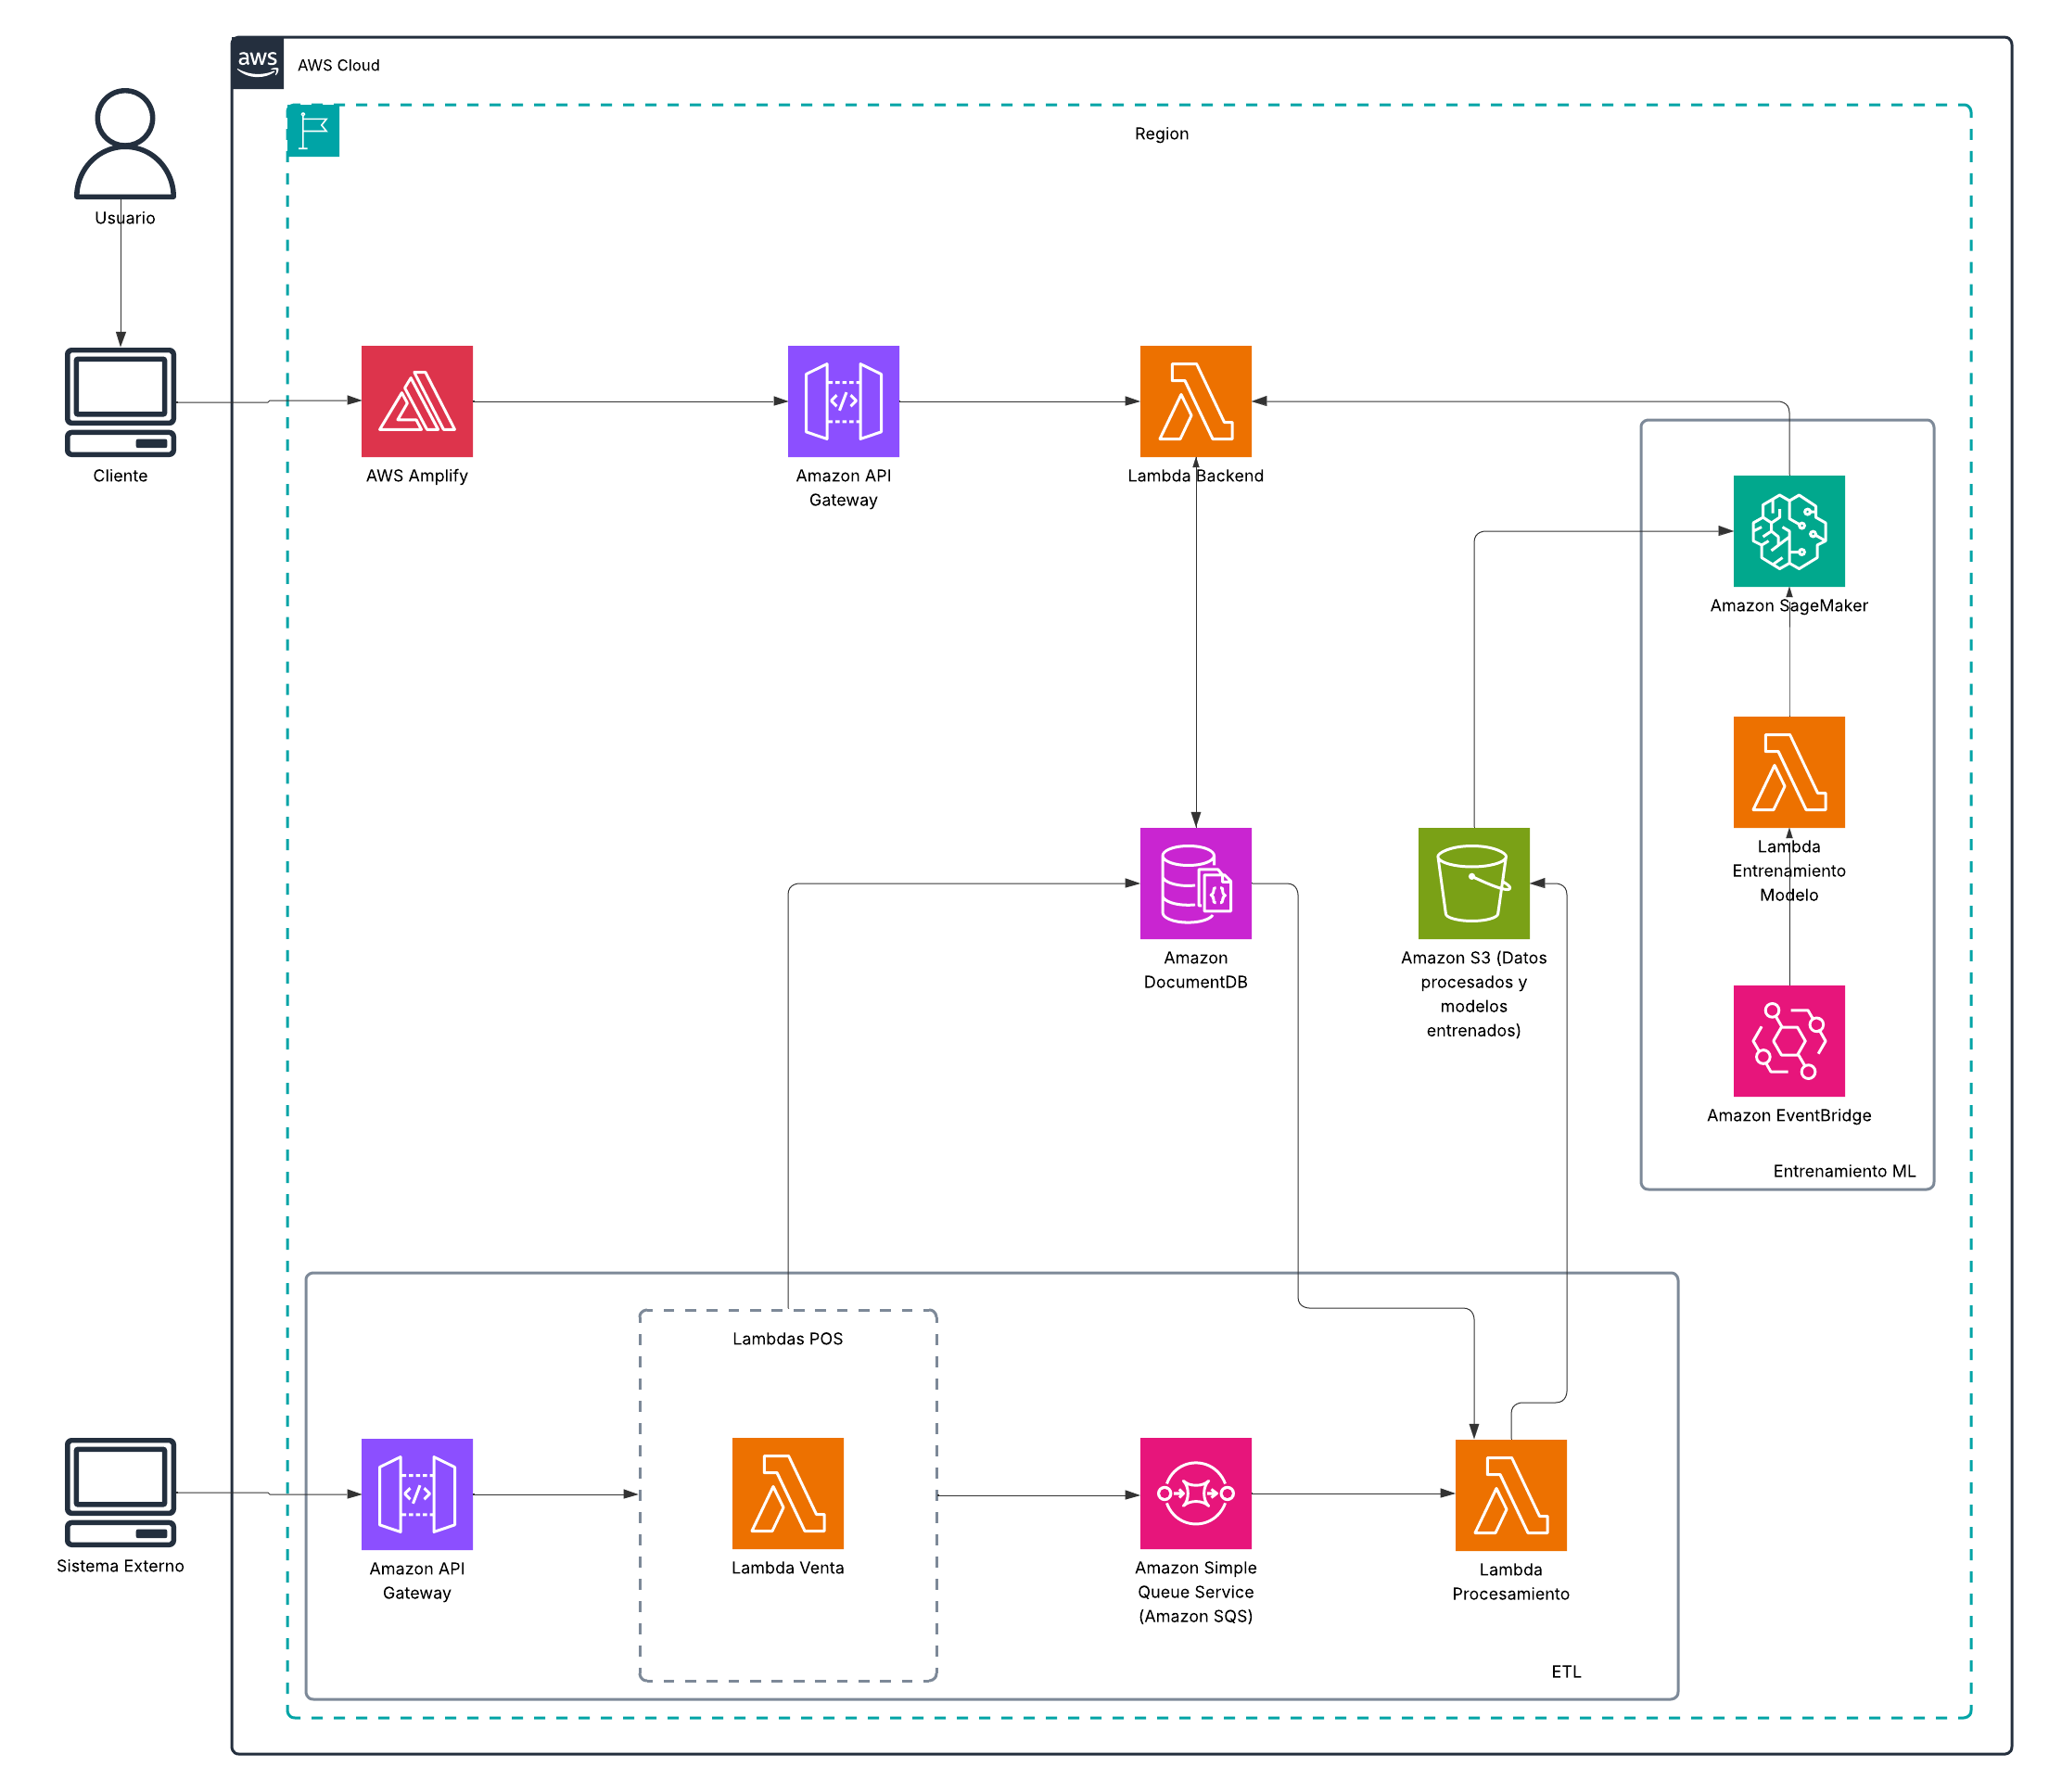
\includegraphics[width=1\textwidth]{images/arquitectura_despliegue.png}
    \caption{Arquitectura de Despliegue y Procesos de SmartStocker}
    \label{fig:arquitectura-despliegue}
\end{figure}

\subsection{Diagrama de Base de datos}\label{sec:arquitectura-base-datos}

Para el diseño de la base de datos, se opto por utilizar DocumentDB, una de las alternativas NoSQL brindadas por AWS, debido a la flexibilidad y capacidades de escalado automatico que esta nos provee, siendo la flexibilidad del schema algo critico dada la necesidad de agregar campos adicionales conforme el proceso de ETL o entrenamiento del modelo de ML lo requieran.

El diseño de la base de datos se organiza alrededor de cinco entidades principales: Usuario, ItemMenu, Ingrediente, Predicción y Venta. La entidad Usuario representa a un negocio dentro de la plataforma. A su vez, la entidad Ingrediente almacena los insumos (nombre, unidad de medida, cantidad en stock y cantidad mínima) y su propietario (userId), mientras que ItemMenu registra los productos ofrecidos (código, nombre, estado activo) y contiene la lista de ingredientes necesarios para cada receta. Esa relación N:M entre ItemMenu e Ingrediente se materializa en la tabla/intersección (el subdocumento de ingredientes) que guarda, por cada par producto-ingrediente, la cantidad\_requerida. La entidad Predicción registra las predicciones de demanda vinculadas a un producto\_id (ItemMenu) con fecha\_prediccion, turno, cantidad\_predicha y el userId que la generó; y la entidad Venta recoge las transacciones reales (número de venta, ítem, producto, cantidad, precio unitario, subtotal, fecha, turno, plataforma, método de pago y estado) asociadas también a un userId. Todos los documentos incluyen timestamps (fecha\_creacion / fecha\_actualizacion) para auditoría.

\begin{figure}[H]
    \centering
    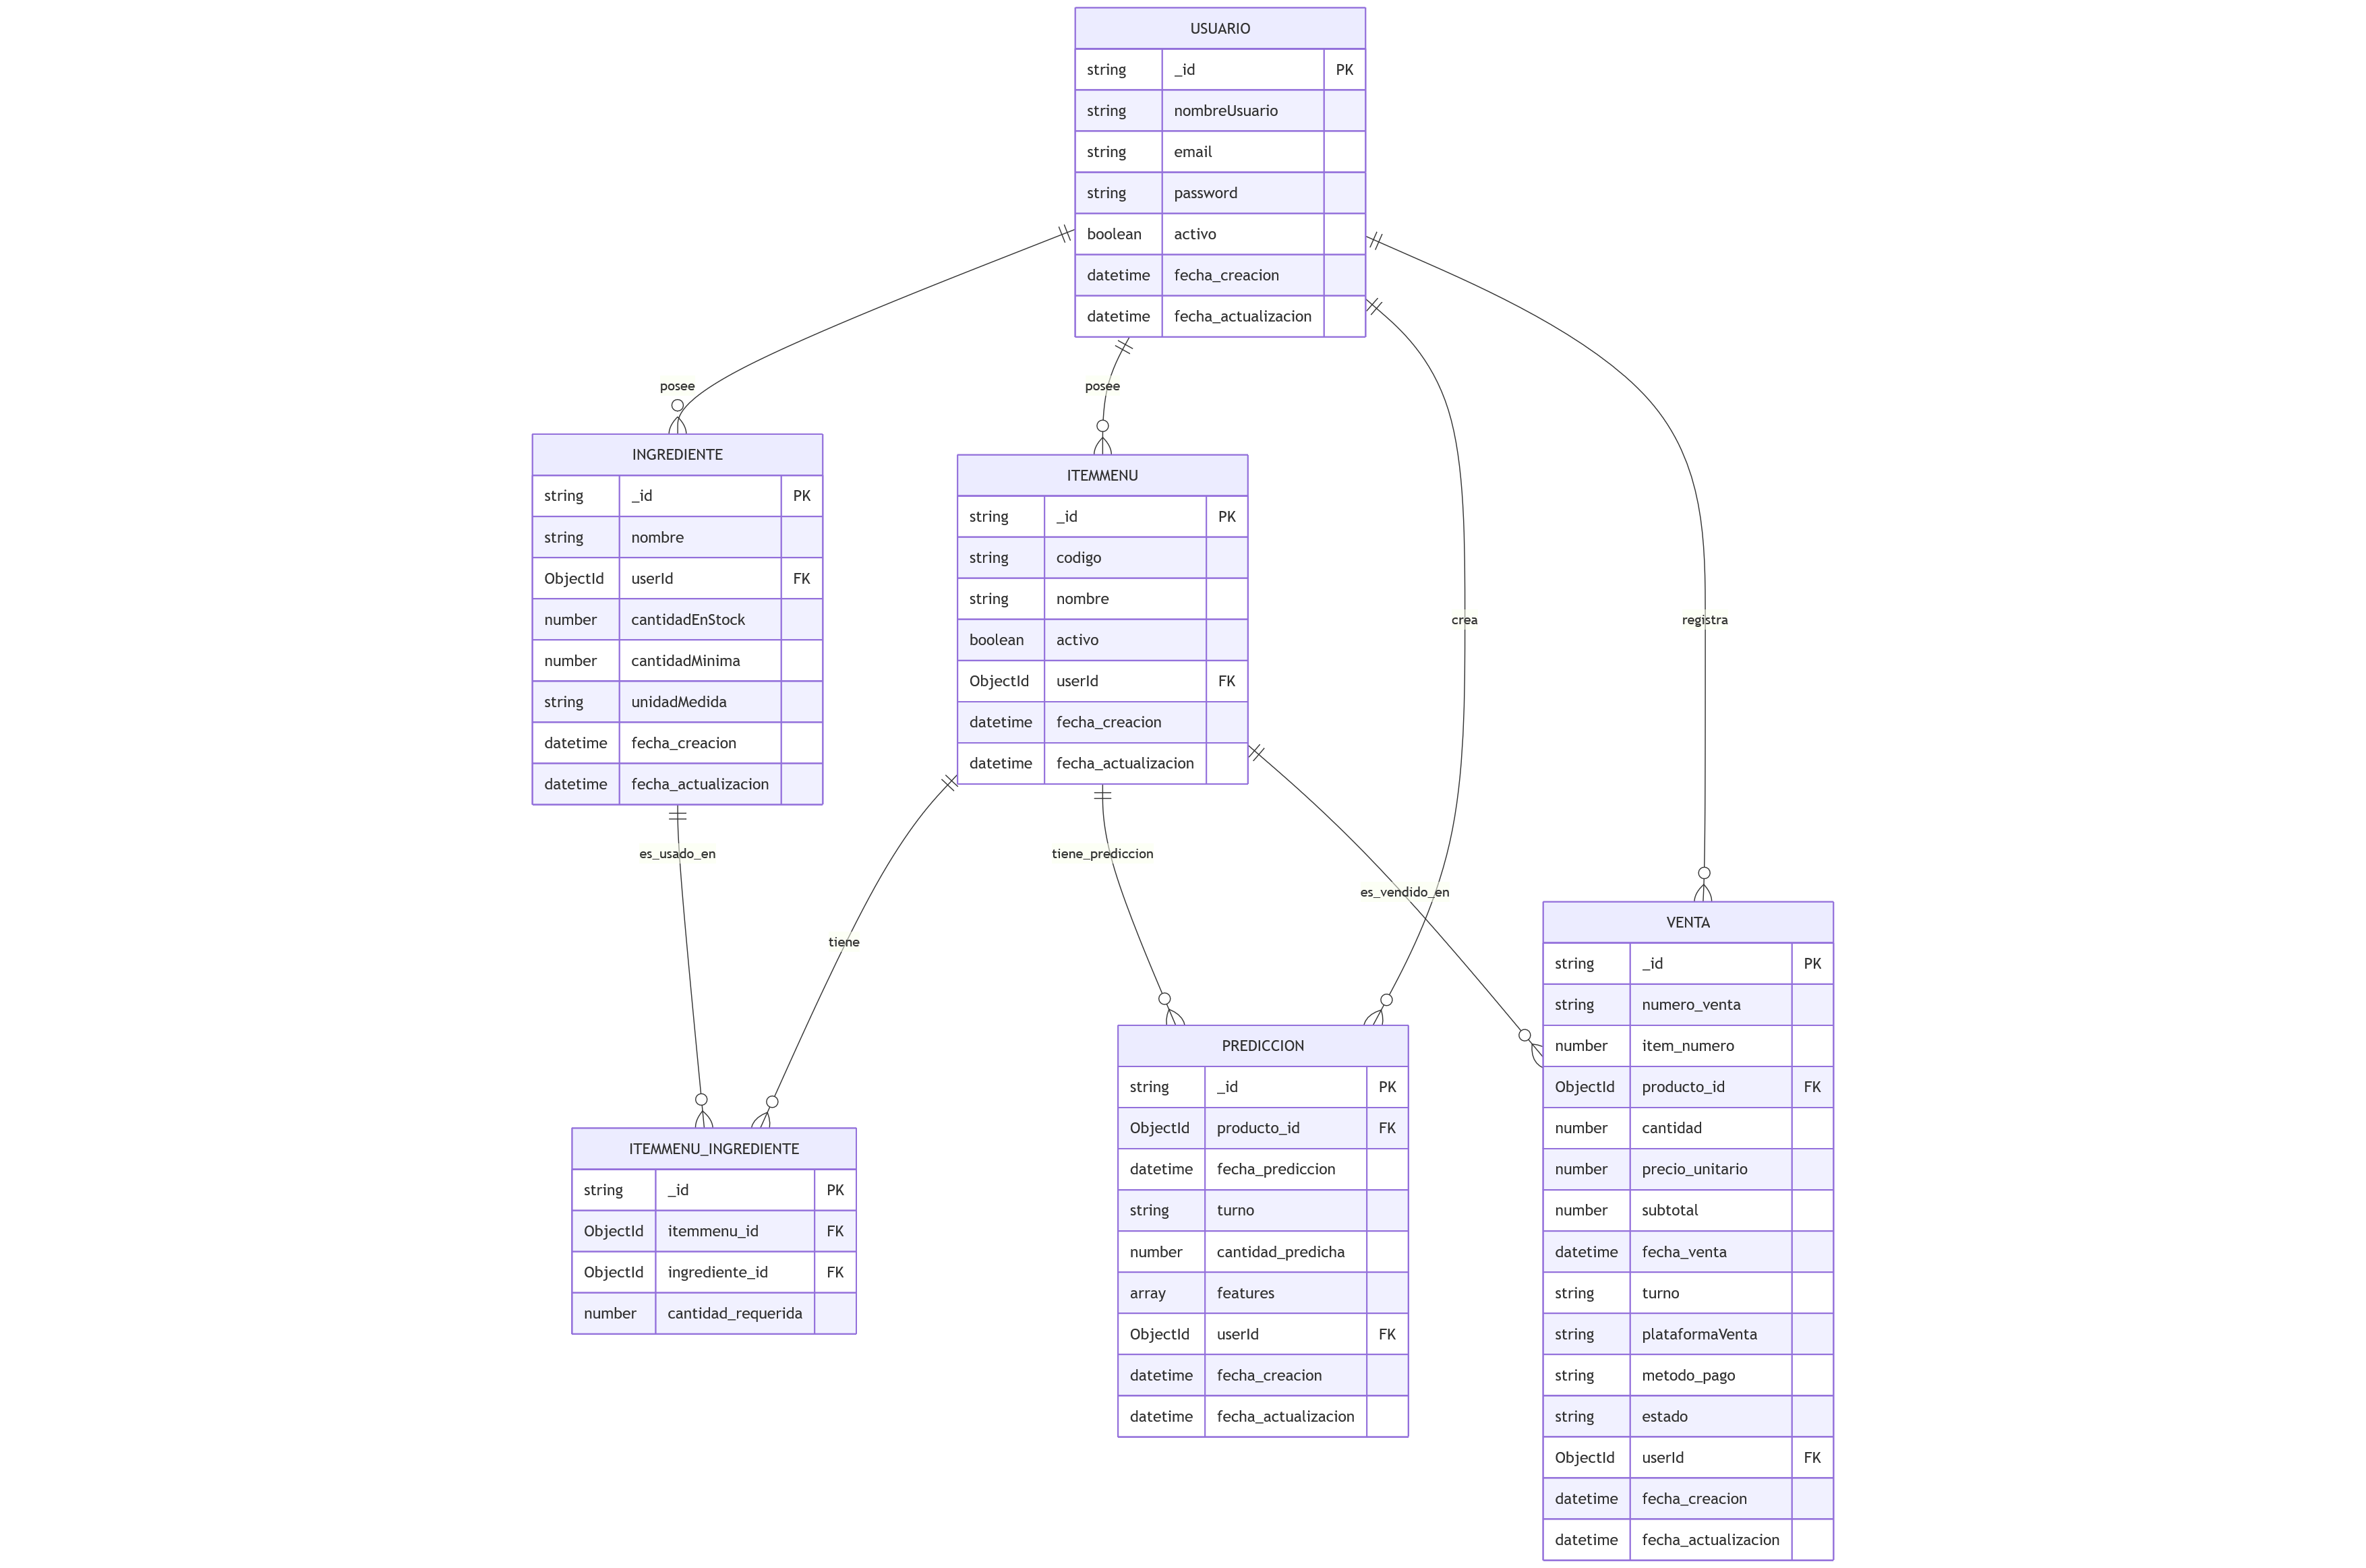
\includegraphics[width=1\textwidth]{images/arquitectura-base-datos.png}
    \caption{Arquitectura de Base de Datos de SmartStocker}
    \label{fig:arquitectura-base-datos}
\end{figure}

\subsection{Pipeline ETL}\label{sec:pipeline-etl}

Con el objetivo de permitir la ingesta automática de las ventas, a fin de actualizar tanto los dashboards visualizados en la aplicación, activar las correspondientes alertas de stock si fuera necesario y disponibilizar la información para el entrenamiento del modelo predictivo, se implementó un pipeline de ETL mediante el cual se procesan las distintas ventas. La primera parte de este proceso es recibir y procesar las ventas que ocurren, para lo cual se diseñaron distintas Lambdas, ajustadas al distinto formato en el que las plataformas pueden enviar los datos de una venta realizada. En estas se analiza la información recibida y en base a ello se genera una nueva entrada en la entidad Ventas. Dado que estas Lambdas estarán atendiendo peticiones de sistemas externos, se decidió que el procesamiento que ocurre en ellas sea lo más rápido y sencillo posible, a fin de devolver una respuesta a la brevedad.

En base a esto, se implementó el uso de AWS SQS, permitiendo de esta forma que el resto de procesamiento requerido para transformar la venta en el dato requerido por el modelo ocurra en una Lambda distinta, que funciona como consumidor de la cola implementada en SQS, donde al finalizar la primer Lambda se encola un mensaje conteniendo el Id de la venta creada en DocumentDb, para que esta sea procesada por el consumidor. Esto nos brinda un procesamiento asincrónico y desacoplado de estas tareas que pueden ser más lentas, y permite que ocurran a un ritmo distinto de la Lambda inicial expuesta al resto de los sistemas de venta.

Esta segunda Lambda se encargará de, en base a la información de la venta y consultas a APIs externas para la obtención de feriados y datos climáticos, generar las features que se considerarán en el entrenamiento del modelo, donde se consideran aspectos relacionados al momento cronológico de la venta, es decir, en qué turno de trabajo ocurre, si se realizó en un feriado, en que semana se hizo, si la venta ocurrió en un fin de semana, pero también se considera el aspecto climático, indicando tanto la estación como el estado climático en ese momento (nublado, despejado, lluvioso), a fin de lograr aspectos estacionales del consumo.
Por último, al finalizar esta Lambda la información procesada es almacenada en un S3, disponible para ser usada al momento de entrenar el modelo.


\subsection{Pipeline Machine Learning}\label{sec:pipeline-machine-learning}

El pipeline de entrenamiento del modelo de machine learning se encuentra implementado mediante el uso de AWS EventBridge, a fin de programar entrenamientos periódicos de forma semanal. El EventBridge disparará un evento que activará una Lambda dedicada al entrenamiento, donde se harán los últimos ajustes a los datos de entrenamiento, se consolidaran los datos de venta, unificando las distintas ventas individuales de acuerdo a la fecha, turno, y producto y se programará la ejecución del entrenamiento en sí, utilizando para esto AWS Sagemaker. Luego del entrenamiento, el modelo será disponibilizado a través de un endpoint, accesible desde la API del backend de la aplicación.

\subsection{Inclusión del Feedback de usuario}\label{sec:inclusion-feedback-usuario}

A fin de incluir el feedback del usuario dentro de las predicciones, se decidió la inclusión de un segundo modelo, cuyo propósito será ajustar la salida del modelo principal, considerando, para cada combinación de producto, turno, y fecha: 

\begin{itemize}
    \item la cantidad de ventas predecida por el modelo.
    \item la cantidad de ventas que efectivamente ocurrieron.
    \item la cantidad de ventas que el usuario espera, brindado como feedback.
\end{itemize}

Este modelo será utilizado para ajustar únicamente las predicciones de productos en las cuales el usuario haya brindado algún feedback, usando únicamente el modelo principal para el resto de productos. Su entrenamiento ocurre en un pipeline similar al del modelo principal, usando como datos de entrenamiento los descritos previamente. A la hora de ejecutar las predicciones, en caso de que haya productos que han recibido feedback por parte del usuario de forma reiterada, esta predicción original será pasada por el segundo modelo, a fin de ajustarla.


	\chapter{Conclusi\'on}\label{conclussions}

\section{Resumen de aportes}

Completar.

\section{Trabajo futuro}

\Nico{Este es un ejemplo de comentario}

Completar.

	\addcontentsline{toc}{chapter}{Bibliograf\'{\i}a}
	\printbibliography{}

	\appendix
	\renewcommand{\appendixname}{Anexo}
\renewcommand{\thechapter}{\Alph{chapter}}

% Comando para iniciar la sección de anexos en el índice
\newcommand{\initappendix}{%
  \addcontentsline{toc}{chapter}{Anexo}%
}

% Comando para cada anexo individual
\newcommand{\anexo}[1]{%
  \refstepcounter{chapter}%
  \chapter*{Anexo \thechapter: #1}%
  \addcontentsline{toc}{section}{Anexo \thechapter: #1}%
  \markboth{Anexo \thechapter: #1}{}%
}

\initappendix

\anexo{Cronograma de Actividades}

En líneas generales, el desarrollo del proyecto ha avanzado conforme a lo planificado. No obstante, se presentó una demora en \ldots, motivo por el cual \ldots. A continuación, se presenta el cronograma actualizado con las tareas realizadas, en curso y replanificadas, que reflejan el estado actual del proyecto.

%\begin{figure}[ht]
%    \centering
%    \includegraphics[width=0.7\textheight]{./././images/Cronograma.png}
%    \caption{Cronograma de actividades.}
%\end{figure} % En las entregas que no son la entrega final, se debe tener al menos un anexo con el cronograma (Gantt)
\anexo{Resultados de la encuesta}

Con el objetivo de comprender los hábitos de consumo en locales gastronómicos y la percepción de los clientes respecto a la disponibilidad de los productos, se realizó una encuesta a más de 150 personas. El propósito de la misma fue poder identificar cómo la falta de stock y la planificación de inventario influyen directamente en la satisfacción y fidelización de los consumidores, un factor clave en el mundo gastronómico.

En cuanto a la frecuencia de consumo, el 69.8\% de los encuestados afirmó visitar locales gastronómicos o pedir por delivery al menos una vez por semana, lo que refleja una relación constante con este tipo de establecimientos.

Respecto a la disponibilidad de productos, el 47.8\%, es decir casi la mitad de los entrevistados señaló que en el último mes le sucedió que el plato o producto deseado no se encontraba disponible. Ahora bien, la falta de stock recurrente sí reflejó tener un impacto notable en la percepción del cliente ya que el 86,8\% indicó que reduciría sus visitas si un local no mantiene la disponibilidad de los platos que ofrece. Además, mientras que el 30,2\% expresó que esta situación le genera desconfianza y afecta negativamente su experiencia, el 62,92\% afirmó que le molesta al menos un poco cuando un plato no está disponible. Si se consideran ambos grupos, puede observarse que más del 93\% de los encuestados experimenta algún grado de molestia o descontento frente a la falta de disponibilidad, lo que evidencia el peso crítico de este factor en la satisfacción del cliente.

Por otra parte, el rol de la planificación de compras resultó clave: el 98,7\% de los participantes coincidió en que una mejor gestión del inventario puede mejorar significativamente el servicio. En la misma línea, el 99,4\% declaró que estaría más dispuesto a regresar a un local que siempre mantenga su menú disponible y con calidad constante, y el 98,7\% lo recomendaría más a terceros.

Finalmente, la encuesta mostró que la falta frecuente de platos afecta directamente la reputación de los locales (71,7\% lo considera un factor muy relevante) y entre las respuestas abiertas, los clientes destacaron como principal fuente de satisfacción la combinación de calidad, disponibilidad, buena atención y relación precio-calidad, confirmando la importancia de un sistema que permita optimizar el control de insumos. % En el caso de tener en cuestas tiene que haber una transcripción de los resultados
\anexo{Transcripción de la entrevista a Alan Turing}

% En el Alan Turing Internet Scrapbook se menciona que Turing ofreció una charla en la radio de la BBC en 1951 
% titulada "Can Computers Think?", y participó en una discusión radiofónica en 1952. 
% Aunque no hay grabaciones conocidas, los guiones (scripts) originales sí están disponibles en el Turing Archive.
% De todas formas, me pareció anecdótico pedirle a un LLM cómo "piensa" que sería esta charla.
% Modelo: GPT5
% Prompt: Piensa cómo sería una entrevista a Alan Turing sobre el paper "Could a computer think?"
\begin{description}[leftmargin=0cm, labelsep=0.5cm]

    \item[\textbf{Entrevistador:}] Profesor Turing, su artículo plantea la pregunta “¿Podría pensar una computadora?”. ¿Cuál diría que es el núcleo de su argumento?

    \item[\textbf{Turing:}] No se trata tanto de si las máquinas pueden pensar, sino de qué entendemos por “pensar”. Propongo desplazar la pregunta hacia algo más verificable: ¿puede una máquina imitar exitosamente el comportamiento inteligente humano al punto de engañar a un observador? Eso es lo que llamo el juego de imitación.

    \item[\textbf{Entrevistador:}] Muchos críticos afirman que las máquinas nunca podrán “pensar” porque carecen de conciencia o emociones.

    \item[\textbf{Turing:}] La objeción de la conciencia es interesante, pero también se aplica a otros seres humanos: no puedo probar que usted sea consciente. Solo puedo observar su comportamiento. Por tanto, es más práctico juzgar la inteligencia por lo que un sistema hace, no por lo que supuestamente es.

    \item[\textbf{Entrevistador:}] En el artículo usted responde a varias objeciones, desde las religiosas hasta las matemáticas. ¿Hay alguna que considere la más difícil de refutar?

    \item[\textbf{Turing:}] Tal vez la objeción de la “infinita variedad” —la idea de que el comportamiento humano es demasiado variado para ser reproducido por reglas finitas. Sin embargo, las matemáticas nos muestran que sistemas finitos pueden generar gran complejidad. La biología también es un buen ejemplo: el código genético es finito, pero produce toda la diversidad de la vida.

    \item[\textbf{Entrevistador:}] Usted menciona que las máquinas podrían aprender. En 1950 eso sonaba muy futurista.

    \item[\textbf{Turing:}] Sí, creo que la programación explícita no es el único camino. Una máquina podría ser diseñada para modificar sus propias instrucciones y mejorar con la experiencia. Sería, en esencia, un aprendiz.

    \item[\textbf{Entrevistador:}] Si mirara hacia el futuro, ¿cómo imagina que evolucionará esta idea?

    \item[\textbf{Turing:}] Confío en que, hacia finales del siglo, las máquinas serán capaces de participar en el juego de imitación con éxito. Tal vez aún habrá debate sobre si “piensan”, pero la práctica hará irrelevante la pregunta: simplemente conviviremos con entidades que actúan inteligentemente.

\end{description}

% Esta entrevista fue real, pero acá dejo una versión acortada
\anexo{Transcripción de la entrevista a Richard Feynman}
\begin{description}[leftmargin=0cm, labelsep=0.5cm]
    \item[\textbf{Interviewer:}] If you get hold of two magnets, and you push them, you can feel this pushing between them. Turn them around the other way, and they slam together. Now, what is it, the feeling between those two magnets?

    \item[\textbf{Feynman:}] What do you mean, "What's the feeling between the two magnets?"

    \item[\textbf{Interviewer:}] There's something there, isn't there? The sensation is that there's something there when you push these two magnets together.

    \item[\textbf{Feynman:}] Listen to my question. What is the meaning when you say that there's a feeling? Of course you feel it. Now what do you want to know?

    \item[\textbf{Interviewer:}] What I want to know is what's going on between these two bits of metal?

    \item[\textbf{Feynman:}] They repel each other.

    \item[\textbf{Interviewer:}] What does that mean, or why are they doing that, or how are they doing that? I think that's a perfectly reasonable question.

    \item[\textbf{Feynman:}] Of course, it's an excellent question. But the problem, you see, when you ask why something happens, how does a person answer why something happens? For example, Aunt Minnie is in the hospital. Why? Because she went out, slipped on the ice, and broke her hip. That satisfies people. It satisfies, but it wouldn't satisfy someone who came from another planet and who knew nothing about why when you break your hip do you go to the hospital. How do you get to the hospital when the hip is broken? Well, because her husband, seeing that her hip was broken, called the hospital up and sent somebody to get her. All that is understood by people. And when you explain a why, you have to be in some framework that you allow something to be true. Otherwise, you're perpetually asking why. Why did the husband call up the hospital? Because the husband is interested in his wife's welfare. Not always, some husbands aren't interested in their wives' welfare when they're drunk, and they're angry.
    \ldots
\end{description} % En el caso de tener entrevistas, se deben poner sus transcripciones
	\newpage
	\listoffigures
	\newpage
	\listoftables
\end{document}
